% Seminarul 6: Selecția modelului și managementul riscului
% Statistica piețelor financiare -- Program de licență, Academia de Studii Economice din București
% GENERAT de latex/build_seminar6.py -- modificați generatorul, nu acest fișier.
% Implicit versiunea pentru studenți; versiunea profesorului este wrapper-ul *_solutions.tex.
\makeatletter\@ifundefined{ifsolutions}{\expandafter\newif\csname ifsolutions\endcsname}{}\makeatother

\newcommand{\coursename}{Statistica piețelor financiare}
\def\sfmlang{ro}
% Preambul comun SFM -- Statistica piețelor financiare / Statistics of Financial Markets (Beamer, 16:9)
% Același design ca MFM. Înainte de % Preambul comun SFM -- Statistica piețelor financiare / Statistics of Financial Markets (Beamer, 16:9)
% Același design ca MFM. Înainte de % Preambul comun SFM -- Statistica piețelor financiare / Statistics of Financial Markets (Beamer, 16:9)
% Același design ca MFM. Înainte de \input{../../latex/preamble} se definește
%   \newcommand{\coursename}{Statistics of Financial Markets}      (EN)
%   \newcommand{\coursename}{Statistica piețelor financiare}       (RO)  și  \def\sfmlang{ro}
% Fișierele .tex se află în EN/Courses, EN/Seminars, RO/Cursuri, RO/Seminarii (două niveluri sub rădăcină).
% Deck-urile sînt generate de latex/build_chapterN.py / build_seminarN.py (vezi latex/sfm_build.py).

\documentclass[9pt, aspectratio=169, t]{beamer}
\providecommand{\coursename}{Statistics of Financial Markets}

% Ensure content fits on slides
\setbeamersize{text margin left=8mm, text margin right=8mm}

%=============================================================================
% THEME AND STYLE CONFIGURATION
%=============================================================================
\usetheme{default}
% Using default theme for clean header/footer control

% Color Palette (matching Redispatch PDF)
\definecolor{MainBlue}{RGB}{26, 58, 110}
\definecolor{AccentBlue}{RGB}{26, 58, 110}
\definecolor{IDAred}{RGB}{205, 0, 0}
\definecolor{DarkGray}{RGB}{51, 51, 51}
\definecolor{MediumGray}{RGB}{128, 128, 128}
\definecolor{LightGray}{RGB}{248, 248, 248}
\definecolor{VeryLightGray}{RGB}{235, 235, 235}
\definecolor{KeynoteGray}{RGB}{218, 218, 218}
\definecolor{SectionGray}{RGB}{120, 120, 120}
\definecolor{FooterGray}{RGB}{100, 100, 100}
\definecolor{Crimson}{RGB}{220, 53, 69}
\definecolor{Forest}{RGB}{46, 125, 50}
\definecolor{Amber}{RGB}{181, 133, 63}
\definecolor{Orange}{RGB}{230, 126, 34}
\definecolor{Purple}{RGB}{142, 68, 173}

% Gradient background (exact Keynote 315° gradient: white to RGB 218,218,218)
\setbeamertemplate{background}{%
    \begin{tikzpicture}[remember picture, overlay]
        \shade[shading=axis, shading angle=315,
        top color=white, bottom color=KeynoteGray]
        (current page.south west) rectangle (current page.north east);
    \end{tikzpicture}%
}
% Fallback solid color for compatibility
\setbeamercolor{background canvas}{bg=}

\setbeamercolor{palette primary}{bg=MainBlue, fg=white}
\setbeamercolor{palette secondary}{bg=MainBlue!85, fg=white}
\setbeamercolor{palette tertiary}{bg=MainBlue!70, fg=white}
\setbeamercolor{structure}{fg=MainBlue}
\setbeamercolor{title}{fg=IDAred}
\setbeamercolor{frametitle}{fg=IDAred, bg=}
\setbeamercolor{block title}{bg=MainBlue, fg=white}
\setbeamercolor{block body}{bg=VeryLightGray, fg=DarkGray}
\setbeamercolor{block title alerted}{bg=Crimson, fg=white}
\setbeamercolor{block body alerted}{bg=Crimson!8, fg=DarkGray}
\setbeamercolor{block title example}{bg=Forest, fg=white}
\setbeamercolor{block body example}{bg=Forest!8, fg=DarkGray}
\setbeamercolor{item}{fg=MainBlue}

% Footer colors (override Madrid theme blue)
\setbeamercolor{author in head/foot}{fg=FooterGray, bg=}
\setbeamercolor{title in head/foot}{fg=FooterGray, bg=}
\setbeamercolor{date in head/foot}{fg=FooterGray, bg=}
\setbeamercolor{section in head/foot}{fg=FooterGray, bg=}
\setbeamercolor{subsection in head/foot}{fg=FooterGray, bg=}

% Bullet styles (apply everywhere including blocks)
\setbeamertemplate{itemize item}{\color{MainBlue}$\boxdot$}
\setbeamertemplate{itemize subitem}{\color{MainBlue}$\blacktriangleright$}
\setbeamertemplate{itemize subsubitem}{\color{MainBlue}\tiny$\bullet$}
\setbeamertemplate{itemize/enumerate body begin}{\normalsize}
\setbeamertemplate{itemize/enumerate subbody begin}{\normalsize}

% Item spacing - compact style
\setlength{\leftmargini}{10pt}       % Level 1: minimal indent
\setlength{\leftmarginii}{10pt}      % Level 2: minimal additional indent
% Compact list spacing (zero extra space before/after lists in blocks)
\makeatletter
\def\@listi{\leftmargin\leftmargini \topsep 0pt \parsep 0pt \itemsep 0pt}
\def\@listii{\leftmargin\leftmarginii \topsep 0pt \parsep 0pt \itemsep 0pt}
\makeatother

\setbeamertemplate{navigation symbols}{}

%=============================================================================
% CUSTOM HEADLINE
%=============================================================================
\setbeamertemplate{headline}{%
    \vskip10pt%
    \hbox to \paperwidth{%
        \hskip0.5cm%
        {\small\color{FooterGray}\renewcommand{\hyperlink}[2]{##2}\insertsectionhead}%
        \hfill%
        \textcolor{FooterGray}{\small\insertframenumber}%
        \hskip0.5cm%
    }%
    \vskip4pt%
    {\color{FooterGray}\hrule height 0.4pt}%
}

%=============================================================================
% CUSTOM FOOTER
%=============================================================================
\usepackage{fontawesome5}

\setbeamertemplate{footline}{%
    {\color{FooterGray}\hrule height 0.4pt}%
    \vskip4pt%
    \hbox to \paperwidth{%
        \hskip0.5cm%
        \textcolor{FooterGray}{\small\coursename}%
        \hfill%
        \raisebox{-0.1em}{%
            \begin{tikzpicture}[x=0.08em, y=0.08em, line width=0.4pt]
                \draw[FooterGray] (0,3) -- (1,4) -- (2,3.5) -- (3,5) -- (4,4) -- (5,6) -- (6,5.5) -- (7,4) -- (8,5) -- (9,7) -- (10,6) -- (11,5) -- (12,6.5) -- (13,8) -- (14,7) -- (15,6) -- (16,7.5) -- (17,9) -- (18,8) -- (19,7) -- (20,8.5) -- (21,10) -- (22,9) -- (23,8) -- (24,9.5);
            \end{tikzpicture}%
        }%
        \hskip0.5cm%
    }%
    \vskip6pt%
}

%=============================================================================
% PACKAGES
%=============================================================================
\usepackage[utf8]{inputenc}
\DeclareUnicodeCharacter{03B1}{\ensuremath{\alpha}}
\usepackage[T1]{fontenc}
\usepackage{amsmath, amssymb, amsthm}
\usepackage{mathtools}
\usepackage{bm}
\usepackage{tikz}
\usetikzlibrary{arrows.meta, positioning, shapes, calc, decorations.pathreplacing, shadings}
\usepackage{booktabs}
\usepackage{multirow}
\usepackage{array}
\usepackage{graphicx}
\usepackage{hyperref}
\usepackage{colortbl}
\usepackage{listings}
\lstset{language=Python, basicstyle=\ttfamily\scriptsize, keywordstyle=\color{MainBlue}\bfseries,
  commentstyle=\color{Forest}, stringstyle=\color{Crimson}, breaklines=true,
  frame=none, backgroundcolor=\color{VeryLightGray}, xleftmargin=2mm}
\hypersetup{colorlinks=true, linkcolor=MainBlue, urlcolor=MainBlue}
\graphicspath{{../../logos/}{../../charts/}{../../photos/}}
\usepackage{xcolor}
\hfuzz=2pt  % Suppress tiny overfull warnings (<2pt)
\vfuzz=2pt  % Suppress tiny vertical overfull warnings (<2pt)

%=============================================================================
% QUANTLET COMMANDS
%   \quantlet{<displayed name>}{<url>}       (generic, compatible with the older SFM decks)
%   \sfmquantlet{Ch_05}{SFM_ch5_garch}       -> https://github.com/danpele/SFM/tree/main/Quantlets/Ch_05/SFM_ch5_garch
%   \qlurl{<folder>} is defined per chapter by the generator (Quantlets/Ch_NN/<folder>)
%=============================================================================
\newcommand{\sfmrepo}{https://github.com/danpele/SFM}
\newcommand{\sfmqlbase}{https://github.com/danpele/SFM/tree/main/Quantlets}
\newcommand{\quantlet}[2]{%
    \hfill\href{#2}{%
        \raisebox{-0.15em}{
\includegraphics[height=0.7em]{ql_logo.png}}%
        \textcolor{MainBlue}{\tiny\ #1}%
    }%
}
\newcommand{\sfmquantlet}[2]{\quantlet{\detokenize{#2}}{\sfmqlbase/#1/#2}}

%=============================================================================
% NOTEBOOKS (Google Colab)
%   \colaburl{notebooks/EN/chapter5_seminar_notebook.ipynb} -> the Colab link of a file in the SFM repo
%   \nb: the chapter notebook (each seminar deck redefines it with \renewcommand)
%=============================================================================
\newcommand{\colaburl}[1]{https://colab.research.google.com/github/danpele/SFM/blob/main/#1}
\newcommand{\nb}{https://colab.research.google.com/github/danpele/SFM/tree/main/notebooks/EN}
\newcommand{\nbname}{notebooks/EN}

%=============================================================================
% SLIDE HELPERS (used by the generators; the same as in MFM)
%=============================================================================
% local font size for list bodies (the preamble forces \normalsize)
\newcommand{\itemsize}[1]{\setbeamertemplate{itemize/enumerate body begin}{#1}\setbeamertemplate{itemize/enumerate subbody begin}{#1}}
\newcommand{\intitle}[1]{{\hypersetup{urlcolor=white}#1}}   % white links inside coloured title bars
\newcommand{\imgcap}[1]{{\scriptsize #1}\\[0.5mm]}          % caption under a photo
\newcommand{\imgcredit}[2]{{\tiny\color{FooterGray}\href{#1}{#2}}}   % image credit: source URL, author/licence
\newcommand{\aiprompt}[1]{{\ttfamily\color{MainBlue}#1}}     % a prompt to an AI assistant

%=============================================================================
% SEMINARS: student version by default; the instructor wrapper *_solutions.tex sets \solutionstrue
%=============================================================================
\makeatletter\@ifundefined{ifsolutions}{\expandafter\newif\csname ifsolutions\endcsname}{}\makeatother
\newcommand{\solonly}[1]{\ifsolutions #1\fi}
\newcommand{\propsub}{\ifsolutions\else\framesubtitle{\ifdefined\sfmlang Rezolvarea se discută la seminar\else Solution discussed in class\fi}\fi}

%=============================================================================
% APPENDIX AND CHAPTER LINKS (latex/appendix_links.py writes the calls; it also re-declares these
% macros before \begin{document}, so the decks compile with or without this preamble block)
%=============================================================================
\providecommand{\sfmapplink}[3]{\hypertarget{#2}{}\hyperlink{#1}{\beamergotobutton{#3}}}
\providecommand{\sfmappback}[2]{\begin{tikzpicture}[remember picture,overlay]\node[anchor=south east] at ([xshift=-3mm,yshift=7mm]current page.south east){\hyperlink{#1}{\beamerreturnbutton{#2}}};\end{tikzpicture}}
\providecommand{\sfmchlink}[2]{\href{#1}{#2}}
\providecommand{\sfmchlinkt}[2]{\href{#1}{\usebeamercolor[fg]{frametitle}#2}}

%=============================================================================
% QUANTINAR COMMAND: link către un curs Quantinar (subiecte avansate)
%=============================================================================
\newcommand{\quantinar}[2]{%
    \href{#2}{%
        \raisebox{-0.15em}{
\includegraphics[height=0.8em]{qr_logo.png}}%
        \textcolor{MainBlue}{\scriptsize\ #1}%
    }%
}

%=============================================================================
% CUSTOM TITLE PAGE
%=============================================================================
\defbeamertemplate*{title page}{hybrid}[1][]
{
    \vspace{0.2cm}
    % Logos row - top header (with clickable links)
    \begin{center}
        \href{https://www.ase.ro}{
\includegraphics[height=1.0cm]{ase_logo.png}}\hspace{0.3cm}%
        \href{https://theida.net}{
\includegraphics[height=1.0cm]{ida_logo.png}}\hspace{0.3cm}%
        \href{https://blockchain-research-center.com}{
\includegraphics[height=1.0cm]{brc_logo.png}}\hspace{0.3cm}%
        \href{https://www.ai4efin.ase.ro}{
\includegraphics[height=1.0cm]{ai4efin_logo.png}}\hspace{0.3cm}%
        \href{https://ipe.ro/new}{
\includegraphics[height=1.0cm]{acad_logo.png}}\hspace{0.3cm}%
        \href{https://www.digital-finance-msca.com}{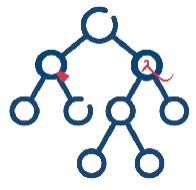
\includegraphics[height=1.0cm]{msca_logo.png}}%
    \end{center}

    \vspace{0.6cm}

    % Main title with Q logos on sides (with clickable links)
    \begin{center}
        \begin{minipage}{0.1\textwidth}
            \centering
            \href{https://quantlet.com}{
\includegraphics[height=1.1cm]{ql_logo.png}}
        \end{minipage}%
        \begin{minipage}{0.78\textwidth}
            \centering
            {\LARGE\bfseries\usebeamercolor[fg]{title}\inserttitle}

            \vspace{0.3cm}

            {\usebeamerfont{subtitle}\usebeamercolor[fg]{title}\insertsubtitle}
        \end{minipage}%
        \begin{minipage}{0.1\textwidth}
            \centering
            \href{https://quantinar.com}{
\includegraphics[height=1.1cm]{qr_logo.png}}
        \end{minipage}
    \end{center}

    \vspace{0.6cm}

    % Authors (left aligned)
    \hspace{0.5cm}{\usebeamerfont{author}\insertauthor}

    \vspace{0.3cm}

    % Institute/Affiliations (left aligned)
    \hspace{0.5cm}\begin{minipage}[t]{0.9\textwidth}
        \raggedright\small\insertinstitute
    \end{minipage}
}

%=============================================================================
% THEOREM ENVIRONMENTS
%=============================================================================
\theoremstyle{definition}
\setbeamertemplate{theorems}[numbered]
\ifdefined\sfmlang
\newtheorem{defn}{Definiție}
\newtheorem{thm}{Teoremă}
\newtheorem{prop}{Propoziție}
\newtheorem{rmk}{Observație}
\else
\newtheorem{defn}{Definition}
\newtheorem{thm}{Theorem}
\newtheorem{prop}{Proposition}
\newtheorem{rmk}{Remark}
\fi

%=============================================================================
% CENTRED MINIPAGE (no extra vertical space)
%=============================================================================
\newenvironment{cminipage}[1]{%
    \par\noindent\hfill\begin{minipage}{#1}\ignorespaces
}{%
    \end{minipage}\hfill\null\par
}

%=============================================================================
% CUSTOM COMMANDS
%=============================================================================
\newcommand{\E}{\mathbb{E}}
\newcommand{\Var}{\text{Var}}
\newcommand{\Cov}{\text{Cov}}
\newcommand{\Corr}{\text{Corr}}
\newcommand{\R}{\mathbb{R}}
\newcommand{\N}{\mathbb{N}}
\newcommand{\Z}{\mathbb{Z}}
\newcommand{\B}{\mathbf{B}}
\newcommand{\imark}{\textcolor{MainBlue}{\textbullet}}
\newcommand{\RMSE}{\text{RMSE}}
\newcommand{\MAE}{\text{MAE}}
\newcommand{\MAPE}{\text{MAPE}}

 se definește
%   \newcommand{\coursename}{Statistics of Financial Markets}      (EN)
%   \newcommand{\coursename}{Statistica piețelor financiare}       (RO)  și  \def\sfmlang{ro}
% Fișierele .tex se află în EN/Courses, EN/Seminars, RO/Cursuri, RO/Seminarii (două niveluri sub rădăcină).
% Deck-urile sînt generate de latex/build_chapterN.py / build_seminarN.py (vezi latex/sfm_build.py).

\documentclass[9pt, aspectratio=169, t]{beamer}
\providecommand{\coursename}{Statistics of Financial Markets}

% Ensure content fits on slides
\setbeamersize{text margin left=8mm, text margin right=8mm}

%=============================================================================
% THEME AND STYLE CONFIGURATION
%=============================================================================
\usetheme{default}
% Using default theme for clean header/footer control

% Color Palette (matching Redispatch PDF)
\definecolor{MainBlue}{RGB}{26, 58, 110}
\definecolor{AccentBlue}{RGB}{26, 58, 110}
\definecolor{IDAred}{RGB}{205, 0, 0}
\definecolor{DarkGray}{RGB}{51, 51, 51}
\definecolor{MediumGray}{RGB}{128, 128, 128}
\definecolor{LightGray}{RGB}{248, 248, 248}
\definecolor{VeryLightGray}{RGB}{235, 235, 235}
\definecolor{KeynoteGray}{RGB}{218, 218, 218}
\definecolor{SectionGray}{RGB}{120, 120, 120}
\definecolor{FooterGray}{RGB}{100, 100, 100}
\definecolor{Crimson}{RGB}{220, 53, 69}
\definecolor{Forest}{RGB}{46, 125, 50}
\definecolor{Amber}{RGB}{181, 133, 63}
\definecolor{Orange}{RGB}{230, 126, 34}
\definecolor{Purple}{RGB}{142, 68, 173}

% Gradient background (exact Keynote 315° gradient: white to RGB 218,218,218)
\setbeamertemplate{background}{%
    \begin{tikzpicture}[remember picture, overlay]
        \shade[shading=axis, shading angle=315,
        top color=white, bottom color=KeynoteGray]
        (current page.south west) rectangle (current page.north east);
    \end{tikzpicture}%
}
% Fallback solid color for compatibility
\setbeamercolor{background canvas}{bg=}

\setbeamercolor{palette primary}{bg=MainBlue, fg=white}
\setbeamercolor{palette secondary}{bg=MainBlue!85, fg=white}
\setbeamercolor{palette tertiary}{bg=MainBlue!70, fg=white}
\setbeamercolor{structure}{fg=MainBlue}
\setbeamercolor{title}{fg=IDAred}
\setbeamercolor{frametitle}{fg=IDAred, bg=}
\setbeamercolor{block title}{bg=MainBlue, fg=white}
\setbeamercolor{block body}{bg=VeryLightGray, fg=DarkGray}
\setbeamercolor{block title alerted}{bg=Crimson, fg=white}
\setbeamercolor{block body alerted}{bg=Crimson!8, fg=DarkGray}
\setbeamercolor{block title example}{bg=Forest, fg=white}
\setbeamercolor{block body example}{bg=Forest!8, fg=DarkGray}
\setbeamercolor{item}{fg=MainBlue}

% Footer colors (override Madrid theme blue)
\setbeamercolor{author in head/foot}{fg=FooterGray, bg=}
\setbeamercolor{title in head/foot}{fg=FooterGray, bg=}
\setbeamercolor{date in head/foot}{fg=FooterGray, bg=}
\setbeamercolor{section in head/foot}{fg=FooterGray, bg=}
\setbeamercolor{subsection in head/foot}{fg=FooterGray, bg=}

% Bullet styles (apply everywhere including blocks)
\setbeamertemplate{itemize item}{\color{MainBlue}$\boxdot$}
\setbeamertemplate{itemize subitem}{\color{MainBlue}$\blacktriangleright$}
\setbeamertemplate{itemize subsubitem}{\color{MainBlue}\tiny$\bullet$}
\setbeamertemplate{itemize/enumerate body begin}{\normalsize}
\setbeamertemplate{itemize/enumerate subbody begin}{\normalsize}

% Item spacing - compact style
\setlength{\leftmargini}{10pt}       % Level 1: minimal indent
\setlength{\leftmarginii}{10pt}      % Level 2: minimal additional indent
% Compact list spacing (zero extra space before/after lists in blocks)
\makeatletter
\def\@listi{\leftmargin\leftmargini \topsep 0pt \parsep 0pt \itemsep 0pt}
\def\@listii{\leftmargin\leftmarginii \topsep 0pt \parsep 0pt \itemsep 0pt}
\makeatother

\setbeamertemplate{navigation symbols}{}

%=============================================================================
% CUSTOM HEADLINE
%=============================================================================
\setbeamertemplate{headline}{%
    \vskip10pt%
    \hbox to \paperwidth{%
        \hskip0.5cm%
        {\small\color{FooterGray}\renewcommand{\hyperlink}[2]{##2}\insertsectionhead}%
        \hfill%
        \textcolor{FooterGray}{\small\insertframenumber}%
        \hskip0.5cm%
    }%
    \vskip4pt%
    {\color{FooterGray}\hrule height 0.4pt}%
}

%=============================================================================
% CUSTOM FOOTER
%=============================================================================
\usepackage{fontawesome5}

\setbeamertemplate{footline}{%
    {\color{FooterGray}\hrule height 0.4pt}%
    \vskip4pt%
    \hbox to \paperwidth{%
        \hskip0.5cm%
        \textcolor{FooterGray}{\small\coursename}%
        \hfill%
        \raisebox{-0.1em}{%
            \begin{tikzpicture}[x=0.08em, y=0.08em, line width=0.4pt]
                \draw[FooterGray] (0,3) -- (1,4) -- (2,3.5) -- (3,5) -- (4,4) -- (5,6) -- (6,5.5) -- (7,4) -- (8,5) -- (9,7) -- (10,6) -- (11,5) -- (12,6.5) -- (13,8) -- (14,7) -- (15,6) -- (16,7.5) -- (17,9) -- (18,8) -- (19,7) -- (20,8.5) -- (21,10) -- (22,9) -- (23,8) -- (24,9.5);
            \end{tikzpicture}%
        }%
        \hskip0.5cm%
    }%
    \vskip6pt%
}

%=============================================================================
% PACKAGES
%=============================================================================
\usepackage[utf8]{inputenc}
\DeclareUnicodeCharacter{03B1}{\ensuremath{\alpha}}
\usepackage[T1]{fontenc}
\usepackage{amsmath, amssymb, amsthm}
\usepackage{mathtools}
\usepackage{bm}
\usepackage{tikz}
\usetikzlibrary{arrows.meta, positioning, shapes, calc, decorations.pathreplacing, shadings}
\usepackage{booktabs}
\usepackage{multirow}
\usepackage{array}
\usepackage{graphicx}
\usepackage{hyperref}
\usepackage{colortbl}
\usepackage{listings}
\lstset{language=Python, basicstyle=\ttfamily\scriptsize, keywordstyle=\color{MainBlue}\bfseries,
  commentstyle=\color{Forest}, stringstyle=\color{Crimson}, breaklines=true,
  frame=none, backgroundcolor=\color{VeryLightGray}, xleftmargin=2mm}
\hypersetup{colorlinks=true, linkcolor=MainBlue, urlcolor=MainBlue}
\graphicspath{{../../logos/}{../../charts/}{../../photos/}}
\usepackage{xcolor}
\hfuzz=2pt  % Suppress tiny overfull warnings (<2pt)
\vfuzz=2pt  % Suppress tiny vertical overfull warnings (<2pt)

%=============================================================================
% QUANTLET COMMANDS
%   \quantlet{<displayed name>}{<url>}       (generic, compatible with the older SFM decks)
%   \sfmquantlet{Ch_05}{SFM_ch5_garch}       -> https://github.com/danpele/SFM/tree/main/Quantlets/Ch_05/SFM_ch5_garch
%   \qlurl{<folder>} is defined per chapter by the generator (Quantlets/Ch_NN/<folder>)
%=============================================================================
\newcommand{\sfmrepo}{https://github.com/danpele/SFM}
\newcommand{\sfmqlbase}{https://github.com/danpele/SFM/tree/main/Quantlets}
\newcommand{\quantlet}[2]{%
    \hfill\href{#2}{%
        \raisebox{-0.15em}{
\includegraphics[height=0.7em]{ql_logo.png}}%
        \textcolor{MainBlue}{\tiny\ #1}%
    }%
}
\newcommand{\sfmquantlet}[2]{\quantlet{\detokenize{#2}}{\sfmqlbase/#1/#2}}

%=============================================================================
% NOTEBOOKS (Google Colab)
%   \colaburl{notebooks/EN/chapter5_seminar_notebook.ipynb} -> the Colab link of a file in the SFM repo
%   \nb: the chapter notebook (each seminar deck redefines it with \renewcommand)
%=============================================================================
\newcommand{\colaburl}[1]{https://colab.research.google.com/github/danpele/SFM/blob/main/#1}
\newcommand{\nb}{https://colab.research.google.com/github/danpele/SFM/tree/main/notebooks/EN}
\newcommand{\nbname}{notebooks/EN}

%=============================================================================
% SLIDE HELPERS (used by the generators; the same as in MFM)
%=============================================================================
% local font size for list bodies (the preamble forces \normalsize)
\newcommand{\itemsize}[1]{\setbeamertemplate{itemize/enumerate body begin}{#1}\setbeamertemplate{itemize/enumerate subbody begin}{#1}}
\newcommand{\intitle}[1]{{\hypersetup{urlcolor=white}#1}}   % white links inside coloured title bars
\newcommand{\imgcap}[1]{{\scriptsize #1}\\[0.5mm]}          % caption under a photo
\newcommand{\imgcredit}[2]{{\tiny\color{FooterGray}\href{#1}{#2}}}   % image credit: source URL, author/licence
\newcommand{\aiprompt}[1]{{\ttfamily\color{MainBlue}#1}}     % a prompt to an AI assistant

%=============================================================================
% SEMINARS: student version by default; the instructor wrapper *_solutions.tex sets \solutionstrue
%=============================================================================
\makeatletter\@ifundefined{ifsolutions}{\expandafter\newif\csname ifsolutions\endcsname}{}\makeatother
\newcommand{\solonly}[1]{\ifsolutions #1\fi}
\newcommand{\propsub}{\ifsolutions\else\framesubtitle{\ifdefined\sfmlang Rezolvarea se discută la seminar\else Solution discussed in class\fi}\fi}

%=============================================================================
% APPENDIX AND CHAPTER LINKS (latex/appendix_links.py writes the calls; it also re-declares these
% macros before \begin{document}, so the decks compile with or without this preamble block)
%=============================================================================
\providecommand{\sfmapplink}[3]{\hypertarget{#2}{}\hyperlink{#1}{\beamergotobutton{#3}}}
\providecommand{\sfmappback}[2]{\begin{tikzpicture}[remember picture,overlay]\node[anchor=south east] at ([xshift=-3mm,yshift=7mm]current page.south east){\hyperlink{#1}{\beamerreturnbutton{#2}}};\end{tikzpicture}}
\providecommand{\sfmchlink}[2]{\href{#1}{#2}}
\providecommand{\sfmchlinkt}[2]{\href{#1}{\usebeamercolor[fg]{frametitle}#2}}

%=============================================================================
% QUANTINAR COMMAND: link către un curs Quantinar (subiecte avansate)
%=============================================================================
\newcommand{\quantinar}[2]{%
    \href{#2}{%
        \raisebox{-0.15em}{
\includegraphics[height=0.8em]{qr_logo.png}}%
        \textcolor{MainBlue}{\scriptsize\ #1}%
    }%
}

%=============================================================================
% CUSTOM TITLE PAGE
%=============================================================================
\defbeamertemplate*{title page}{hybrid}[1][]
{
    \vspace{0.2cm}
    % Logos row - top header (with clickable links)
    \begin{center}
        \href{https://www.ase.ro}{
\includegraphics[height=1.0cm]{ase_logo.png}}\hspace{0.3cm}%
        \href{https://theida.net}{
\includegraphics[height=1.0cm]{ida_logo.png}}\hspace{0.3cm}%
        \href{https://blockchain-research-center.com}{
\includegraphics[height=1.0cm]{brc_logo.png}}\hspace{0.3cm}%
        \href{https://www.ai4efin.ase.ro}{
\includegraphics[height=1.0cm]{ai4efin_logo.png}}\hspace{0.3cm}%
        \href{https://ipe.ro/new}{
\includegraphics[height=1.0cm]{acad_logo.png}}\hspace{0.3cm}%
        \href{https://www.digital-finance-msca.com}{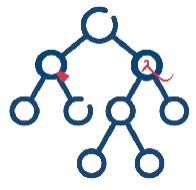
\includegraphics[height=1.0cm]{msca_logo.png}}%
    \end{center}

    \vspace{0.6cm}

    % Main title with Q logos on sides (with clickable links)
    \begin{center}
        \begin{minipage}{0.1\textwidth}
            \centering
            \href{https://quantlet.com}{
\includegraphics[height=1.1cm]{ql_logo.png}}
        \end{minipage}%
        \begin{minipage}{0.78\textwidth}
            \centering
            {\LARGE\bfseries\usebeamercolor[fg]{title}\inserttitle}

            \vspace{0.3cm}

            {\usebeamerfont{subtitle}\usebeamercolor[fg]{title}\insertsubtitle}
        \end{minipage}%
        \begin{minipage}{0.1\textwidth}
            \centering
            \href{https://quantinar.com}{
\includegraphics[height=1.1cm]{qr_logo.png}}
        \end{minipage}
    \end{center}

    \vspace{0.6cm}

    % Authors (left aligned)
    \hspace{0.5cm}{\usebeamerfont{author}\insertauthor}

    \vspace{0.3cm}

    % Institute/Affiliations (left aligned)
    \hspace{0.5cm}\begin{minipage}[t]{0.9\textwidth}
        \raggedright\small\insertinstitute
    \end{minipage}
}

%=============================================================================
% THEOREM ENVIRONMENTS
%=============================================================================
\theoremstyle{definition}
\setbeamertemplate{theorems}[numbered]
\ifdefined\sfmlang
\newtheorem{defn}{Definiție}
\newtheorem{thm}{Teoremă}
\newtheorem{prop}{Propoziție}
\newtheorem{rmk}{Observație}
\else
\newtheorem{defn}{Definition}
\newtheorem{thm}{Theorem}
\newtheorem{prop}{Proposition}
\newtheorem{rmk}{Remark}
\fi

%=============================================================================
% CENTRED MINIPAGE (no extra vertical space)
%=============================================================================
\newenvironment{cminipage}[1]{%
    \par\noindent\hfill\begin{minipage}{#1}\ignorespaces
}{%
    \end{minipage}\hfill\null\par
}

%=============================================================================
% CUSTOM COMMANDS
%=============================================================================
\newcommand{\E}{\mathbb{E}}
\newcommand{\Var}{\text{Var}}
\newcommand{\Cov}{\text{Cov}}
\newcommand{\Corr}{\text{Corr}}
\newcommand{\R}{\mathbb{R}}
\newcommand{\N}{\mathbb{N}}
\newcommand{\Z}{\mathbb{Z}}
\newcommand{\B}{\mathbf{B}}
\newcommand{\imark}{\textcolor{MainBlue}{\textbullet}}
\newcommand{\RMSE}{\text{RMSE}}
\newcommand{\MAE}{\text{MAE}}
\newcommand{\MAPE}{\text{MAPE}}

 se definește
%   \newcommand{\coursename}{Statistics of Financial Markets}      (EN)
%   \newcommand{\coursename}{Statistica piețelor financiare}       (RO)  și  \def\sfmlang{ro}
% Fișierele .tex se află în EN/Courses, EN/Seminars, RO/Cursuri, RO/Seminarii (două niveluri sub rădăcină).
% Deck-urile sînt generate de latex/build_chapterN.py / build_seminarN.py (vezi latex/sfm_build.py).

\documentclass[9pt, aspectratio=169, t]{beamer}
\providecommand{\coursename}{Statistics of Financial Markets}

% Ensure content fits on slides
\setbeamersize{text margin left=8mm, text margin right=8mm}

%=============================================================================
% THEME AND STYLE CONFIGURATION
%=============================================================================
\usetheme{default}
% Using default theme for clean header/footer control

% Color Palette (matching Redispatch PDF)
\definecolor{MainBlue}{RGB}{26, 58, 110}
\definecolor{AccentBlue}{RGB}{26, 58, 110}
\definecolor{IDAred}{RGB}{205, 0, 0}
\definecolor{DarkGray}{RGB}{51, 51, 51}
\definecolor{MediumGray}{RGB}{128, 128, 128}
\definecolor{LightGray}{RGB}{248, 248, 248}
\definecolor{VeryLightGray}{RGB}{235, 235, 235}
\definecolor{KeynoteGray}{RGB}{218, 218, 218}
\definecolor{SectionGray}{RGB}{120, 120, 120}
\definecolor{FooterGray}{RGB}{100, 100, 100}
\definecolor{Crimson}{RGB}{220, 53, 69}
\definecolor{Forest}{RGB}{46, 125, 50}
\definecolor{Amber}{RGB}{181, 133, 63}
\definecolor{Orange}{RGB}{230, 126, 34}
\definecolor{Purple}{RGB}{142, 68, 173}

% Gradient background (exact Keynote 315° gradient: white to RGB 218,218,218)
\setbeamertemplate{background}{%
    \begin{tikzpicture}[remember picture, overlay]
        \shade[shading=axis, shading angle=315,
        top color=white, bottom color=KeynoteGray]
        (current page.south west) rectangle (current page.north east);
    \end{tikzpicture}%
}
% Fallback solid color for compatibility
\setbeamercolor{background canvas}{bg=}

\setbeamercolor{palette primary}{bg=MainBlue, fg=white}
\setbeamercolor{palette secondary}{bg=MainBlue!85, fg=white}
\setbeamercolor{palette tertiary}{bg=MainBlue!70, fg=white}
\setbeamercolor{structure}{fg=MainBlue}
\setbeamercolor{title}{fg=IDAred}
\setbeamercolor{frametitle}{fg=IDAred, bg=}
\setbeamercolor{block title}{bg=MainBlue, fg=white}
\setbeamercolor{block body}{bg=VeryLightGray, fg=DarkGray}
\setbeamercolor{block title alerted}{bg=Crimson, fg=white}
\setbeamercolor{block body alerted}{bg=Crimson!8, fg=DarkGray}
\setbeamercolor{block title example}{bg=Forest, fg=white}
\setbeamercolor{block body example}{bg=Forest!8, fg=DarkGray}
\setbeamercolor{item}{fg=MainBlue}

% Footer colors (override Madrid theme blue)
\setbeamercolor{author in head/foot}{fg=FooterGray, bg=}
\setbeamercolor{title in head/foot}{fg=FooterGray, bg=}
\setbeamercolor{date in head/foot}{fg=FooterGray, bg=}
\setbeamercolor{section in head/foot}{fg=FooterGray, bg=}
\setbeamercolor{subsection in head/foot}{fg=FooterGray, bg=}

% Bullet styles (apply everywhere including blocks)
\setbeamertemplate{itemize item}{\color{MainBlue}$\boxdot$}
\setbeamertemplate{itemize subitem}{\color{MainBlue}$\blacktriangleright$}
\setbeamertemplate{itemize subsubitem}{\color{MainBlue}\tiny$\bullet$}
\setbeamertemplate{itemize/enumerate body begin}{\normalsize}
\setbeamertemplate{itemize/enumerate subbody begin}{\normalsize}

% Item spacing - compact style
\setlength{\leftmargini}{10pt}       % Level 1: minimal indent
\setlength{\leftmarginii}{10pt}      % Level 2: minimal additional indent
% Compact list spacing (zero extra space before/after lists in blocks)
\makeatletter
\def\@listi{\leftmargin\leftmargini \topsep 0pt \parsep 0pt \itemsep 0pt}
\def\@listii{\leftmargin\leftmarginii \topsep 0pt \parsep 0pt \itemsep 0pt}
\makeatother

\setbeamertemplate{navigation symbols}{}

%=============================================================================
% CUSTOM HEADLINE
%=============================================================================
\setbeamertemplate{headline}{%
    \vskip10pt%
    \hbox to \paperwidth{%
        \hskip0.5cm%
        {\small\color{FooterGray}\renewcommand{\hyperlink}[2]{##2}\insertsectionhead}%
        \hfill%
        \textcolor{FooterGray}{\small\insertframenumber}%
        \hskip0.5cm%
    }%
    \vskip4pt%
    {\color{FooterGray}\hrule height 0.4pt}%
}

%=============================================================================
% CUSTOM FOOTER
%=============================================================================
\usepackage{fontawesome5}

\setbeamertemplate{footline}{%
    {\color{FooterGray}\hrule height 0.4pt}%
    \vskip4pt%
    \hbox to \paperwidth{%
        \hskip0.5cm%
        \textcolor{FooterGray}{\small\coursename}%
        \hfill%
        \raisebox{-0.1em}{%
            \begin{tikzpicture}[x=0.08em, y=0.08em, line width=0.4pt]
                \draw[FooterGray] (0,3) -- (1,4) -- (2,3.5) -- (3,5) -- (4,4) -- (5,6) -- (6,5.5) -- (7,4) -- (8,5) -- (9,7) -- (10,6) -- (11,5) -- (12,6.5) -- (13,8) -- (14,7) -- (15,6) -- (16,7.5) -- (17,9) -- (18,8) -- (19,7) -- (20,8.5) -- (21,10) -- (22,9) -- (23,8) -- (24,9.5);
            \end{tikzpicture}%
        }%
        \hskip0.5cm%
    }%
    \vskip6pt%
}

%=============================================================================
% PACKAGES
%=============================================================================
\usepackage[utf8]{inputenc}
\DeclareUnicodeCharacter{03B1}{\ensuremath{\alpha}}
\usepackage[T1]{fontenc}
\usepackage{amsmath, amssymb, amsthm}
\usepackage{mathtools}
\usepackage{bm}
\usepackage{tikz}
\usetikzlibrary{arrows.meta, positioning, shapes, calc, decorations.pathreplacing, shadings}
\usepackage{booktabs}
\usepackage{multirow}
\usepackage{array}
\usepackage{graphicx}
\usepackage{hyperref}
\usepackage{colortbl}
\usepackage{listings}
\lstset{language=Python, basicstyle=\ttfamily\scriptsize, keywordstyle=\color{MainBlue}\bfseries,
  commentstyle=\color{Forest}, stringstyle=\color{Crimson}, breaklines=true,
  frame=none, backgroundcolor=\color{VeryLightGray}, xleftmargin=2mm}
\hypersetup{colorlinks=true, linkcolor=MainBlue, urlcolor=MainBlue}
\graphicspath{{../../logos/}{../../charts/}{../../photos/}}
\usepackage{xcolor}
\hfuzz=2pt  % Suppress tiny overfull warnings (<2pt)
\vfuzz=2pt  % Suppress tiny vertical overfull warnings (<2pt)

%=============================================================================
% QUANTLET COMMANDS
%   \quantlet{<displayed name>}{<url>}       (generic, compatible with the older SFM decks)
%   \sfmquantlet{Ch_05}{SFM_ch5_garch}       -> https://github.com/danpele/SFM/tree/main/Quantlets/Ch_05/SFM_ch5_garch
%   \qlurl{<folder>} is defined per chapter by the generator (Quantlets/Ch_NN/<folder>)
%=============================================================================
\newcommand{\sfmrepo}{https://github.com/danpele/SFM}
\newcommand{\sfmqlbase}{https://github.com/danpele/SFM/tree/main/Quantlets}
\newcommand{\quantlet}[2]{%
    \hfill\href{#2}{%
        \raisebox{-0.15em}{
\includegraphics[height=0.7em]{ql_logo.png}}%
        \textcolor{MainBlue}{\tiny\ #1}%
    }%
}
\newcommand{\sfmquantlet}[2]{\quantlet{\detokenize{#2}}{\sfmqlbase/#1/#2}}

%=============================================================================
% NOTEBOOKS (Google Colab)
%   \colaburl{notebooks/EN/chapter5_seminar_notebook.ipynb} -> the Colab link of a file in the SFM repo
%   \nb: the chapter notebook (each seminar deck redefines it with \renewcommand)
%=============================================================================
\newcommand{\colaburl}[1]{https://colab.research.google.com/github/danpele/SFM/blob/main/#1}
\newcommand{\nb}{https://colab.research.google.com/github/danpele/SFM/tree/main/notebooks/EN}
\newcommand{\nbname}{notebooks/EN}

%=============================================================================
% SLIDE HELPERS (used by the generators; the same as in MFM)
%=============================================================================
% local font size for list bodies (the preamble forces \normalsize)
\newcommand{\itemsize}[1]{\setbeamertemplate{itemize/enumerate body begin}{#1}\setbeamertemplate{itemize/enumerate subbody begin}{#1}}
\newcommand{\intitle}[1]{{\hypersetup{urlcolor=white}#1}}   % white links inside coloured title bars
\newcommand{\imgcap}[1]{{\scriptsize #1}\\[0.5mm]}          % caption under a photo
\newcommand{\imgcredit}[2]{{\tiny\color{FooterGray}\href{#1}{#2}}}   % image credit: source URL, author/licence
\newcommand{\aiprompt}[1]{{\ttfamily\color{MainBlue}#1}}     % a prompt to an AI assistant

%=============================================================================
% SEMINARS: student version by default; the instructor wrapper *_solutions.tex sets \solutionstrue
%=============================================================================
\makeatletter\@ifundefined{ifsolutions}{\expandafter\newif\csname ifsolutions\endcsname}{}\makeatother
\newcommand{\solonly}[1]{\ifsolutions #1\fi}
\newcommand{\propsub}{\ifsolutions\else\framesubtitle{\ifdefined\sfmlang Rezolvarea se discută la seminar\else Solution discussed in class\fi}\fi}

%=============================================================================
% APPENDIX AND CHAPTER LINKS (latex/appendix_links.py writes the calls; it also re-declares these
% macros before \begin{document}, so the decks compile with or without this preamble block)
%=============================================================================
\providecommand{\sfmapplink}[3]{\hypertarget{#2}{}\hyperlink{#1}{\beamergotobutton{#3}}}
\providecommand{\sfmappback}[2]{\begin{tikzpicture}[remember picture,overlay]\node[anchor=south east] at ([xshift=-3mm,yshift=7mm]current page.south east){\hyperlink{#1}{\beamerreturnbutton{#2}}};\end{tikzpicture}}
\providecommand{\sfmchlink}[2]{\href{#1}{#2}}
\providecommand{\sfmchlinkt}[2]{\href{#1}{\usebeamercolor[fg]{frametitle}#2}}

%=============================================================================
% QUANTINAR COMMAND: link către un curs Quantinar (subiecte avansate)
%=============================================================================
\newcommand{\quantinar}[2]{%
    \href{#2}{%
        \raisebox{-0.15em}{
\includegraphics[height=0.8em]{qr_logo.png}}%
        \textcolor{MainBlue}{\scriptsize\ #1}%
    }%
}

%=============================================================================
% CUSTOM TITLE PAGE
%=============================================================================
\defbeamertemplate*{title page}{hybrid}[1][]
{
    \vspace{0.2cm}
    % Logos row - top header (with clickable links)
    \begin{center}
        \href{https://www.ase.ro}{
\includegraphics[height=1.0cm]{ase_logo.png}}\hspace{0.3cm}%
        \href{https://theida.net}{
\includegraphics[height=1.0cm]{ida_logo.png}}\hspace{0.3cm}%
        \href{https://blockchain-research-center.com}{
\includegraphics[height=1.0cm]{brc_logo.png}}\hspace{0.3cm}%
        \href{https://www.ai4efin.ase.ro}{
\includegraphics[height=1.0cm]{ai4efin_logo.png}}\hspace{0.3cm}%
        \href{https://ipe.ro/new}{
\includegraphics[height=1.0cm]{acad_logo.png}}\hspace{0.3cm}%
        \href{https://www.digital-finance-msca.com}{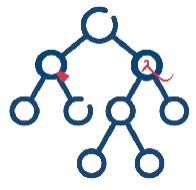
\includegraphics[height=1.0cm]{msca_logo.png}}%
    \end{center}

    \vspace{0.6cm}

    % Main title with Q logos on sides (with clickable links)
    \begin{center}
        \begin{minipage}{0.1\textwidth}
            \centering
            \href{https://quantlet.com}{
\includegraphics[height=1.1cm]{ql_logo.png}}
        \end{minipage}%
        \begin{minipage}{0.78\textwidth}
            \centering
            {\LARGE\bfseries\usebeamercolor[fg]{title}\inserttitle}

            \vspace{0.3cm}

            {\usebeamerfont{subtitle}\usebeamercolor[fg]{title}\insertsubtitle}
        \end{minipage}%
        \begin{minipage}{0.1\textwidth}
            \centering
            \href{https://quantinar.com}{
\includegraphics[height=1.1cm]{qr_logo.png}}
        \end{minipage}
    \end{center}

    \vspace{0.6cm}

    % Authors (left aligned)
    \hspace{0.5cm}{\usebeamerfont{author}\insertauthor}

    \vspace{0.3cm}

    % Institute/Affiliations (left aligned)
    \hspace{0.5cm}\begin{minipage}[t]{0.9\textwidth}
        \raggedright\small\insertinstitute
    \end{minipage}
}

%=============================================================================
% THEOREM ENVIRONMENTS
%=============================================================================
\theoremstyle{definition}
\setbeamertemplate{theorems}[numbered]
\ifdefined\sfmlang
\newtheorem{defn}{Definiție}
\newtheorem{thm}{Teoremă}
\newtheorem{prop}{Propoziție}
\newtheorem{rmk}{Observație}
\else
\newtheorem{defn}{Definition}
\newtheorem{thm}{Theorem}
\newtheorem{prop}{Proposition}
\newtheorem{rmk}{Remark}
\fi

%=============================================================================
% CENTRED MINIPAGE (no extra vertical space)
%=============================================================================
\newenvironment{cminipage}[1]{%
    \par\noindent\hfill\begin{minipage}{#1}\ignorespaces
}{%
    \end{minipage}\hfill\null\par
}

%=============================================================================
% CUSTOM COMMANDS
%=============================================================================
\newcommand{\E}{\mathbb{E}}
\newcommand{\Var}{\text{Var}}
\newcommand{\Cov}{\text{Cov}}
\newcommand{\Corr}{\text{Corr}}
\newcommand{\R}{\mathbb{R}}
\newcommand{\N}{\mathbb{N}}
\newcommand{\Z}{\mathbb{Z}}
\newcommand{\B}{\mathbf{B}}
\newcommand{\imark}{\textcolor{MainBlue}{\textbullet}}
\newcommand{\RMSE}{\text{RMSE}}
\newcommand{\MAE}{\text{MAE}}
\newcommand{\MAPE}{\text{MAPE}}



\newcommand{\qlurl}[1]{https://github.com/danpele/SFM/tree/main/Quantlets/Ch_06/#1}
\renewcommand{\nb}{\colaburl{notebooks/EN/chapter6_seminar_notebook.ipynb}}
\renewcommand{\nbname}{chapter6\_seminar\_notebook.ipynb}
% left column: full width in the student version, narrower next to the solution
\newcommand{\taskw}{\ifsolutions 0.47\textwidth\else 0.96\textwidth\fi}
\newcommand{\solw}{\ifsolutions 0.49\textwidth\else 0pt\fi}

% Clickable citations (DOIs verified via Crossref)

\newcommand{\refFHH}{\href{https://doi.org/10.1007/978-3-030-13751-9}{Franke, Härdle \& Hafner (2019)}}
\newcommand{\refFHHex}{\href{https://doi.org/10.1007/978-3-642-33929-5}{Borak, Härdle \& López-Cabrera (2013)}}
\newcommand{\refTsay}{\href{https://doi.org/10.1002/9780470644560}{Tsay (2010)}}
\newcommand{\refBox}{\href{https://doi.org/10.1080/01621459.1976.10480949}{Box (1976)}}
\newcommand{\refAkaike}{\href{https://doi.org/10.1109/TAC.1974.1100705}{Akaike (1974)}}
\newcommand{\refSchwarz}{\href{https://doi.org/10.1214/aos/1176344136}{Schwarz (1978)}}
\newcommand{\refKL}{\href{https://doi.org/10.1214/aoms/1177729694}{Kullback \& Leibler (1951)}}
\newcommand{\refBA}{\href{https://doi.org/10.1177/0049124104268644}{Burnham \& Anderson (2004)}}
\newcommand{\refBAbook}{\href{https://doi.org/10.1007/b97636}{Burnham \& Anderson (2002)}}
\newcommand{\refStone}{\href{https://doi.org/10.1111/j.2517-6161.1977.tb01603.x}{Stone (1977)}}
\newcommand{\refHT}{\href{https://doi.org/10.1093/biomet/76.2.297}{Hurvich \& Tsai (1989)}}
\newcommand{\refWilks}{\href{https://doi.org/10.1214/aoms/1177732360}{Wilks (1938)}}
\newcommand{\refSL}{\href{https://doi.org/10.1080/01621459.1987.10478472}{Self \& Liang (1987)}}
\newcommand{\refVuong}{\href{https://doi.org/10.2307/1912557}{Vuong (1989)}}
\newcommand{\refPearson}{\href{https://doi.org/10.1080/14786440009463897}{Pearson (1900)}}
\newcommand{\refSmirnov}{\href{https://doi.org/10.1214/aoms/1177730256}{Smirnov (1948)}}
\newcommand{\refLilliefors}{\href{https://doi.org/10.1080/01621459.1967.10482916}{Lilliefors (1967)}}
\newcommand{\refAD}{\href{https://doi.org/10.1214/aoms/1177729437}{Anderson \& Darling (1952)}}
\newcommand{\refADb}{\href{https://doi.org/10.1080/01621459.1954.10501232}{Anderson \& Darling (1954)}}
\newcommand{\refCramer}{\href{https://doi.org/10.1080/03461238.1928.10416862}{Cramér (1928)}}
\newcommand{\refStephens}{\href{https://doi.org/10.1080/01621459.1974.10480196}{Stephens (1974)}}
\newcommand{\refSGQ}{\href{https://doi.org/10.1007/BF02613687}{Stute et al.\ (1993)}}
\newcommand{\refHansen}{\href{https://doi.org/10.2307/2527081}{Hansen (1994)}}
\newcommand{\refNelson}{\href{https://doi.org/10.2307/2938260}{Nelson (1991)}}
\newcommand{\refKon}{\href{https://doi.org/10.1111/j.1540-6261.1984.tb03865.x}{Kon (1984)}}
\newcommand{\refBN}{\href{https://doi.org/10.1111/1467-9469.00045}{Barndorff-Nielsen (1997)}}
\newcommand{\refEK}{\href{https://doi.org/10.2307/3318481}{Eberlein \& Keller (1995)}}
\newcommand{\refKupiec}{\href{https://doi.org/10.3905/jod.1995.407942}{Kupiec (1995)}}
\newcommand{\refGR}{\href{https://doi.org/10.1198/016214506000001437}{Gneiting \& Raftery (2007)}}
\newcommand{\refAG}{\href{https://doi.org/10.1198/073500106000000332}{Amisano \& Giacomini (2007)}}
\newcommand{\refDPD}{\href{https://doi.org/10.1016/j.jeconom.2011.04.001}{Diks, Panchenko \& van Dijk (2011)}}
\newcommand{\refHoeting}{\href{https://doi.org/10.1214/ss/1009212519}{Hoeting et al.\ (1999)}}
\newcommand{\refDanielsson}{\href{https://doi.org/10.1016/j.jfs.2016.02.002}{Danielsson et al.\ (2016)}}
\newcommand{\refKerkhof}{\href{https://doi.org/10.1016/j.jbankfin.2009.07.025}{Kerkhof, Melenberg \& Schumacher (2010)}}
\newcommand{\refCont}{\href{https://doi.org/10.1080/713665670}{Cont (2001)}}
\newcommand{\refPeleA}{\href{https://doi.org/10.3390/e19050226}{Pele, Lazar \& Dufour (2017)}}
\newcommand{\refPeleB}{\href{https://doi.org/10.3390/e21121204}{Pele, Lazar \& Mazurencu-Marinescu-Pele (2019)}}
\newcommand{\refWang}{\href{https://doi.org/10.1038/s41586-023-06221-2}{Wang et al.\ (2023)}}

\title[Statistica piețelor financiare]{Statistica piețelor financiare}
\subtitle{Seminarul 6: Selecția modelului și managementul riscului\ifsolutions\ (versiunea profesorului)\fi}
\author[D.T. Pele]{Daniel Traian PELE}
\institute{Academia de Studii Economice din București\\
IDA Institute Digital Assets\\
Blockchain Research Center\\
AI4EFin Artificial Intelligence for Energy Finance\\
Academia Română, Institutul de Prognoză Economică\\
MSCA Digital Finance}
\date{}

%=============================================================================
\providecommand{\sfmapplink}[3]{\hypertarget{#2}{}\hyperlink{#1}{\beamergotobutton{#3}}}  % APPLINKS-MACROS
\providecommand{\sfmappback}[2]{\begin{tikzpicture}[remember picture,overlay]\node[anchor=south east] at ([xshift=-3mm,yshift=7mm]current page.south east){\hyperlink{#1}{\beamerreturnbutton{#2}}};\end{tikzpicture}}  % APPLINKS-MACROS
\providecommand{\sfmchlink}[2]{\href{#1}{#2}}  % APPLINKS-MACROS
\providecommand{\sfmchlinkt}[2]{\href{#1}{\usebeamercolor[fg]{frametitle}#2}}  % APPLINKS-MACROS
\begin{document}
%=============================================================================

{
\setbeamertemplate{headline}{}
\setbeamertemplate{footline}{}
\begin{frame}[noframenumbering]
    \titlepage
\end{frame}
}
% BEGIN-ACRONYMS (generat de latex/acronyms.py; nu editati manual)
\begin{frame}{Acronime folosite în acest material}
\setbeamertemplate{itemize/enumerate body begin}{\tiny}
\begin{columns}[T]
\begin{column}{0.49\textwidth}
\begin{itemize}\setlength{\itemsep}{0pt}
    \item \textbf{AD}: Anderson–Darling (test) (testul Anderson–Darling)
    \item \textbf{AI}: Artificial Intelligence (inteligență artificială)
    \item \textbf{AIC}: Akaike Information Criterion (criteriul informațional Akaike)
    \item \textbf{BET}: Bucharest Exchange Trading (index) (indicele de referință al Bursei de Valori București)
    \item \textbf{BIC}: Bayesian Information Criterion (criteriul informațional bayesian)
    \item \textbf{EDF}: Empirical Distribution Function (funcția de repartiție empirică)
    \item \textbf{EODHD}: EOD Historical Data (market-data provider) (furnizor de date de piață)
    \item \textbf{ES}: Expected Shortfall (pierderea așteptată în coadă)
    \item \textbf{GED}: Generalised Error Distribution (distribuția erorii generalizate)
    \item \textbf{KS}: Kolmogorov–Smirnov (test) (testul Kolmogorov–Smirnov)
    \item \textbf{LR}: Likelihood Ratio (raportul de verosimilitate)
    \item \textbf{ML}: Maximum Likelihood (verosimilitate maximă)
    \item \textbf{NIG}: Normal Inverse Gaussian (distribution) (distribuția Normală invers Gaussiană)
\end{itemize}
\end{column}
\begin{column}{0.49\textwidth}
\begin{itemize}\setlength{\itemsep}{0pt}
    \item \textbf{QQ}: Quantile–Quantile (plot) (graficul cuantilă–cuantilă)
\end{itemize}
\end{column}
\end{columns}
\end{frame}
% END-ACRONYMS

\begin{frame}{Întrebarea de azi și traseul}
\itemsize{\small}
\begin{itemize}
    \item \textbf{Întrebarea}: dintre mai multe distribuții candidate pentru randamentele zilnice, pe care o alegem și de unde știm că este suficient de bună pentru VaR 1\%?
    \begin{itemize}
        \item seminarul are loc \textbf{înaintea} Cursului 6: secțiunea „Noțiuni necesare azi” dă toate definițiile folosite în cerințe
    \end{itemize}
    \item Traseul
    \begin{itemize}
        \item Partea A: AIC, BIC, ponderi Akaike, teste ale raportului de verosimilitate, un test KS și depășiri VaR, pe hîrtie
        \item Partea B: alegerea modelului pe BET, S\&P 500, DAX, Bitcoin și Banca Transilvania, fiecare cu o întrebare de interpretare
        \item Partea C: o întrebare deschisă pentru proiect și un răspuns AI de verificat
    \end{itemize}
    \item Notebook-ul de azi: \href{\nb}{deschideți notebook-ul seminarului în Google Colab}; fiecare cerință indică secțiunea din notebook
    \item Nu se predă nimic: seminarul este pentru exercițiu; rezolvările cerințelor [Propus] se discută la seminar
\end{itemize}
\end{frame}

\begin{frame}{Harta exercițiilor}
\itemsize{\small}
\begin{center}
\footnotesize
\begin{tabular}{>{\raggedright\arraybackslash}p{1.1cm}>{\raggedright\arraybackslash}p{7.5cm}>{\raggedright\arraybackslash}p{1.9cm}>{\raggedright\arraybackslash}p{1.4cm}}
\toprule
\textbf{Cerința} & \textbf{Întrebarea} & \textbf{Tipul} & \textbf{Model} \\
\midrule
A1, A2 & care model are cel mai mic AIC și BIC și cît de puternice sînt dovezile? & Rezolvat, Propus & A1 \\
A3, A4 & este modelul mai larg dintre două modele imbricate semnificativ mai bun? & Rezolvat, Propus & A3 \\
A5, A6 & trece un eșantion mic un test KS, cu parametri cunoscuți și cu parametri estimați? & Rezolvat, Propus & A5 \\
A7, A8 & VaR 1\% în două modele; sînt depășirile prea multe sau prea puține? & Rezolvat, Propus & A7 \\
B1, B2 & care distribuție se potrivește cel mai bine randamentelor BET, DAX și Bitcoin? & Rezolvat, Propus & B1 \\
B3, B4 & trec cele mai bune modele un test de concordanță? sînt două zile TLV erori de date? & Rezolvat, Propus & B3 \\
B5, B6 & care model nimerește VaR 1\% în afara eșantionului? & Rezolvat, Propus & B5 \\
C1, C2 & se schimbă în timp cel mai bun model? ce este greșit într-un răspuns AI? & Propus & B1, A3 \\
\bottomrule
\end{tabular}
\end{center}
\begin{itemize}
    \item \textbf{[Rezolvat]}: rezolvarea completă în slide-uri și în notebook, un model de urmat; \textbf{[Propus]}: îl rezolvați voi, după model
\end{itemize}
\end{frame}

\begin{frame}{Datele folosite}
\itemsize{\small}
\begin{center}
\footnotesize
\begin{tabular}{llll}
\toprule
\textbf{Seria} & \textbf{Sursa} & \textbf{Prețul folosit} & \textbf{Perioada} \\
\midrule
BET, S\&P 500, DAX & EODHD & close & 2000--2026 \\
Bitcoin & EODHD & close, 7 zile pe săptămînă & 2014--2026 \\
Banca Transilvania (TLV) & EODHD & close ajustat & 2010--2026 \\
\bottomrule
\end{tabular}
\end{center}
\begin{itemize}
    \item Randamente logaritmice zilnice în \%: $r_t = 100\,(\ln P_t - \ln P_{t-1})$; weekendurile și închiderile repetate din zilele libere se elimină (cu excepția Bitcoin)
    \item Șase modele candidate: Normală, Student-t, skewed-t, GED, amestec Normal cu două componente, NIG
    \item În notebook: \texttt{returns('bet')}, \texttt{fit\_model('NIG', x)}; nu este nevoie de cont sau de cheie
\end{itemize}
\end{frame}


%=============================================================================
\section{Noțiuni necesare azi}
%=============================================================================

\begin{frame}{Noțiuni necesare azi (1/5): verosimilitatea și candidații}
\itemsize{\small}
\begin{itemize}
    \item Randamentele $r_1, \dots, r_n$ i.i.d.\ (independente și identic distribuite), cu densitatea $f(r; \theta)$
    \begin{itemize}
        \item log-verosimilitatea $\ell(\theta) = \sum_t \ln f(r_t; \theta)$; estimarea ML (maximum likelihood, verosimilitate maximă) $\hat\theta$ o maximizează
        \item Normală: $\ell(\hat\theta) = -\frac{n}{2}[\ln(2\pi\hat\sigma^2) + 1]$ cu $\hat\sigma^2 = \frac{1}{n}\sum_t (r_t - \bar r)^2$
    \end{itemize}
    \item Candidații și numărul lor de parametri $k$
    \begin{itemize}
        \item Normală (2); Student-t (3: $\nu$, locație, scală); skewed-t (4: adaugă asimetria $\lambda$; $\lambda = 0$ dă Student-t)
        \item GED, generalised error distribution (distribuția erorii generalizate) (3: forma $\beta$; $\beta = 2$ dă legea Normală); amestec Normal cu două componente (5); NIG, normal inverse Gaussian (4)
    \end{itemize}
    \item Cu cît cozile datelor sînt mai groase, cu atît modelul Normal pierde mai mult în $\ell$
\end{itemize}
\end{frame}

\begin{frame}{Noțiuni necesare azi (2/5): AIC, BIC, ponderi Akaike}
\itemsize{\small}
\begin{itemize}
    \item $\mathrm{AIC} = -2\ell(\hat\theta) + 2k$ (Akaike information criterion, criteriul informațional Akaike); $\mathrm{BIC} = -2\ell(\hat\theta) + k\ln n$ (Bayesian information criterion, criteriul informațional bayesian)
    \begin{itemize}
        \item mai mic este mai bine; contează doar diferențele pe aceleași date; BIC penalizează mai mult parametrii cînd $\ln n > 2$, adică $n > 7$
    \end{itemize}
    \item $\Delta_i = \mathrm{AIC}_i - \min_j \mathrm{AIC}_j$; ponderea Akaike $w_i = e^{-\Delta_i/2}/\sum_j e^{-\Delta_j/2}$
    \begin{itemize}
        \item reguli practice \refBA: $\Delta \le 2$ sprijin substanțial; $4$--$7$ considerabil mai puțin; $> 10$ practic niciunul
    \end{itemize}
    \item AIC nu este un test: nu există valoare $p$ și nici „semnificație”
\end{itemize}
\end{frame}

\begin{frame}{Noțiuni necesare azi (3/5): testul raportului de verosimilitate}
\itemsize{\small}
\begin{itemize}
    \item Modelul 0 este \textbf{imbricat} în modelul 1 dacă este modelul 1 cu unii parametri fixați (Student-t = skewed-t cu $\lambda = 0$)
    \begin{itemize}
        \item $LR = 2[\ell_1(\hat\theta_1) - \ell_0(\hat\theta_0)] \approx \chi^2(k_1 - k_0)$ sub $H_0$ (Wilks)
        \item valori critice la 5\%: $\chi^2_{0{,}95}(1) = 3{,}84$, $\chi^2_{0{,}95}(2) = 5{,}99$
    \end{itemize}
    \item \textbf{Frontiera}: Normală în Student-t înseamnă $1/\nu = 0$, marginea spațiului parametrilor
    \begin{itemize}
        \item atunci $LR$ urmează un amestec 50:50 de 0 și $\chi^2(1)$ \refSL: valoarea critică la 5\% $2{,}71$, valoarea $p$ = jumătate din cea $\chi^2(1)$
    \end{itemize}
    \item Perechi neimbricate (Student-t vs GED): fără test LR; folosiți AIC sau testul Vuong
\end{itemize}
\end{frame}

\begin{frame}{Noțiuni necesare azi (4/5): teste de concordanță}
\itemsize{\small}
\begin{itemize}
    \item EDF (empirical distribution function, funcția de repartiție empirică) $F_n(x) = \frac{1}{n}\#\{t: r_t \le x\}$; funcția de repartiție a modelului $F$
    \begin{itemize}
        \item \textbf{KS} (Kolmogorov--Smirnov): $D_n = \max_i \max\{i/n - u_{(i)},\ u_{(i)} - (i-1)/n\}$ cu $u_{(i)} = F(r_{(i)})$ pe datele ordonate
        \item \textbf{CvM} (Cramér--von Mises) și \textbf{AD} (Anderson--Darling) integrează pătratul distanței; AD o ponderează cu $1/[F(1-F)]$: se uită la cozi
    \end{itemize}
    \item Valori critice KS la 5\%
    \begin{itemize}
        \item $F$ complet cunoscută: $n = 5$: $0{,}563$; $n = 6$: $0{,}519$; $n$ mare: $1{,}358/\sqrt{n}$
        \item media și varianța estimate din aceleași date (Lilliefors): $n = 5$: $0{,}354$; $n = 6$: $0{,}333$; alte modele: bootstrap parametric
    \end{itemize}
    \item Un grafic QQ pune datele ordonate față de cuantilele modelului $F^{-1}((i - 0{,}5)/n)$: cozile care se îndepărtează de dreaptă sînt greșite
\end{itemize}
\end{frame}

\begin{frame}{Noțiuni necesare azi (5/5): VaR, depășiri, în afara eșantionului}
\itemsize{\footnotesize}
\begin{itemize}
    \item $\mathrm{VaR}_{1\%} = -q_{1\%}$, pierderea zilnică depășită cu probabilitatea 1\%; Normală: $\mathrm{VaR}_{1\%} = -(\mu - 2{,}326\sigma)$
    \begin{itemize}
        \item ES 2,5\% (expected shortfall): pierderea medie dincolo de $q_{2{,}5\%}$; Normală: $-\mu + \sigma\varphi(z_{0{,}025})/0{,}025$
    \end{itemize}
    \item \textbf{Depășire}: o zi cu $r_t < -\mathrm{VaR}$; pentru un model corect, $x \sim \mathrm{Binomial}(n; 0{,}01)$
    \begin{itemize}
        \item testul Kupiec: $LR_{uc} = -2[\ell_0 - \ell_1]$, $\ell_0 = (n - x)\ln 0{,}99 + x\ln 0{,}01$, $\ell_1 = (n - x)\ln(1 - \hat p) + x\ln\hat p$, $\hat p = x/n$; comparăm cu $\chi^2(1)$
    \end{itemize}
    \item \textbf{În afara eșantionului}: ajustăm pînă la o dată, evaluăm după ea
    \begin{itemize}
        \item scorul logaritmic: media lui $\ln f(r_t; \hat\theta)$ pe zilele de test (mai mare este mai bine); pierderea pinball a cuantilei de 1\% $q$: media lui $(0{,}01 - \mathbf{1}\{r_t < q\})(r_t - q)$ (mai mic este mai bine)
    \end{itemize}
\end{itemize}
\end{frame}


%=============================================================================
\section{Partea A: calcule pe hîrtie}
%=============================================================================

\begin{frame}{A1: patru modele pentru S\&P 500 [Rezolvat]}
\itemsize{\scriptsize}
\begin{columns}[T]
\begin{column}{0.47\textwidth}
\begin{block}{Cerință}
\begin{itemize}
    \item S\&P 500, ultimele $n = 1000$ de zile de tranzacționare (2022--2026); log-verosimilitățile maximizate:
    \item Normală: $\ell = -1400{,}9$, $k = 2$
    \item Student-t: $\ell = -1314{,}7$, $k = 3$
    \item skewed-t: $\ell = -1313{,}8$, $k = 4$
    \item GED: $\ell = -1322{,}6$, $k = 3$
    \item 1. Calculați AIC și BIC ($\ln 1000 = 6{,}908$) pentru fiecare model.
    \item 2. Calculați $\Delta$AIC și ponderile Akaike.
    \item 3. Spuneți ce model alege fiecare criteriu și cît de puternice sînt dovezile.
    \item Raportați: un tabel cu patru rînduri și două fraze.
\end{itemize}
\end{block}
\end{column}
\begin{column}{0.49\textwidth}
\begin{exampleblock}{Rezolvare}
\begin{itemize}
    \item 1. AIC: Normală $2805{,}8$, Student-t $2635{,}4$, skewed-t $2635{,}6$, GED $2651{,}2$; BIC: $2815{,}6$, $2650{,}1$, $2655{,}2$, $2665{,}9$
    \item 2. $\Delta$AIC: $170{,}4$, $0{,}0$, $0{,}2$, $15{,}8$; $e^{-\Delta/2}$: $0{,}000$, $1{,}000$, $0{,}905$, $0{,}000$; ponderi $0{,}000$, $0{,}525$, $0{,}475$, $0{,}000$
    \item 3. AIC: Student-t și skewed-t la egalitate ($\Delta = 0{,}2$); BIC: Student-t, la $5{,}1$ puncte; modelul Normal și GED nu au niciun sprijin.
\end{itemize}
\end{exampleblock}
\end{column}
\end{columns}
\end{frame}

\begin{frame}{A2: patru modele pentru Bitcoin [Propus]}
\propsub
\itemsize{\scriptsize}
\begin{columns}[T]
\begin{column}{\taskw}
\begin{block}{Cerință}
\begin{itemize}
    \item Bitcoin, ultimele $n = 1000$ de zile (2023--2026); log-verosimilitățile maximizate: Model: A1.
    \item Normală: $\ell = -2328{,}0$, $k = 2$
    \item Student-t: $\ell = -2262{,}0$, $k = 3$
    \item NIG: $\ell = -2258{,}4$, $k = 4$
    \item amestec Normal: $\ell = -2262{,}3$, $k = 5$
    \item 1. Calculați AIC, BIC, $\Delta$AIC și ponderile Akaike.
    \item 2. Spuneți dacă AIC și BIC aleg același model.
    \item 3. Explicați de ce amestecul Normal, cu cei mai mulți parametri, nu cîștigă.
    \item Raportați: un tabel cu patru rînduri și două fraze.
\end{itemize}
\end{block}
\end{column}
\begin{column}{\solw}
\solonly{%
\begin{exampleblock}{Rezolvare}
\begin{itemize}
    \item 1. AIC: $4660{,}0$, $4530{,}0$, $4524{,}8$, $4534{,}6$; BIC: $4669{,}8$, $4544{,}7$, $4544{,}4$, $4559{,}1$; ponderi $0{,}000$, $0{,}069$, $0{,}924$, $0{,}007$
    \item 2. AIC: NIG ($\Delta$ al Student-t $5{,}2$); BIC: NIG și Student-t aproape la egalitate ($\Delta$BIC $0{,}3$).
    \item 3. $\ell$ al său nu este mai mare decît al Student-t și plătește pentru doi parametri în plus: un amestec Normal are cozi Normale (subțiri).
\end{itemize}
\end{exampleblock}
}
\end{column}
\end{columns}
\end{frame}

\begin{frame}{A3: este necesară asimetria? Ajunge legea Normală? [Rezolvat]}
\itemsize{\scriptsize}
\begin{columns}[T]
\begin{column}{0.47\textwidth}
\begin{block}{Cerință}
\begin{itemize}
    \item Folosiți log-verosimilitățile din A1 (S\&P 500, $n = 1000$).
    \item 1. Testați Student-t ($H_0$: $\lambda = 0$) față de skewed-t cu un test al raportului de verosimilitate la 5\%.
    \item 2. Testați legea Normală ($H_0$: $\beta = 2$) față de GED.
    \item 3. Comparați decizia LR de la pasul 1 cu verdictul AIC din A1.
    \item Raportați: două valori $LR$, două decizii și o frază.
\end{itemize}
\end{block}
\end{column}
\begin{column}{0.49\textwidth}
\begin{exampleblock}{Rezolvare}
\begin{itemize}
    \item 1. $LR = 2(-1313{,}8 - (-1314{,}7)) = 1{,}8 < 3{,}84$, $p = 0{,}18$: nu respingem $\lambda = 0$
    \item 2. $LR = 2(-1322{,}6 - (-1400{,}9)) = 156{,}6$, $p <0{,}001$: respingem legea Normală
    \item 3. Concordante: AIC găsește cele două modele t la egalitate; testul LR nu găsește un cîștig semnificativ din $\lambda$. Pentru perechi imbricate, AIC preferă modelul mai larg exact cînd $LR > 2$ pe parametru în plus.
\end{itemize}
\end{exampleblock}
\end{column}
\end{columns}
\end{frame}

\begin{frame}{A4: un test la frontieră [Propus]}
\propsub
\itemsize{\scriptsize}
\begin{columns}[T]
\begin{column}{\taskw}
\begin{block}{Cerință}
\begin{itemize}
    \item Folosiți log-verosimilitățile din A2 (Bitcoin, $n = 1000$). Model: A3.
    \item 1. Calculați $LR$ pentru legea Normală inclusă în Student-t.
    \item 2. Explicați de ce legea sub $H_0$ nu este $\chi^2(1)$ și dați valoarea critică corectă la 5\%.
    \item 3. Spuneți dacă un test LR poate compara Student-t cu NIG.
    \item Raportați: o valoare $LR$, o valoare critică și două fraze.
\end{itemize}
\end{block}
\end{column}
\begin{column}{\solw}
\solonly{%
\begin{exampleblock}{Rezolvare}
\begin{itemize}
    \item 1. $LR = 2(-2262{,}0 - (-2328{,}0)) = 132{,}0$
    \item 2. $H_0$ este $1/\nu = 0$, pe marginea lui $1/\nu \ge 0$: legea este un amestec 50:50 de 0 și $\chi^2(1)$, valoarea critică $\chi^2_{0{,}90}(1) = 2{,}71$; respingem legea Normală oricum.
    \item 3. Nu: niciunul nu este caz particular al celuilalt; folosiți AIC sau testul Vuong.
\end{itemize}
\end{exampleblock}
}
\end{column}
\end{columns}
\end{frame}

\begin{frame}{A5: KS pe cinci randamente [Rezolvat]}
\itemsize{\scriptsize}
\begin{columns}[T]
\begin{column}{0.47\textwidth}
\begin{block}{Cerință}
\begin{itemize}
    \item Randamente zilnice (\%): $-2{,}1$; $-0{,}4$; $0{,}3$; $0{,}9$; $1{,}6$.
    \item 1. Calculați $D_5$ față de $N(0, 1)$ și comparați-l cu valoarea critică la 5\% $0{,}563$.
    \item 2. Estimați $\hat\mu$ și $\hat\sigma$ (împărțitor $n$), calculați $D_5$ față de $N(\hat\mu, \hat\sigma^2)$ și comparați-l cu valoarea Lilliefors $0{,}354$.
    \item 3. Explicați de ce valoarea critică Lilliefors este mai mică.
    \item Raportați: două valori $D_5$, două decizii, o frază.
\end{itemize}
\end{block}
\end{column}
\begin{column}{0.49\textwidth}
\begin{exampleblock}{Rezolvare}
\begin{itemize}
    \item 1. $u_{(i)} = \Phi(r_{(i)})$: $0{,}018$; $0{,}345$; $0{,}618$; $0{,}816$; $0{,}945$; cea mai mare distanță $D_5 = 0{,}218 < 0{,}563$: nu respingem
    \item 2. $\hat\mu = 0{,}060$, $\hat\sigma = 1{,}266$; $z_{(i)}$: $-1{,}71$; $-0{,}36$; $0{,}19$; $0{,}66$; $1{,}22$; $u_{(i)}$: $0{,}044$; $0{,}358$; $0{,}575$; $0{,}747$; $0{,}888$; $D_5 = 0{,}175 < 0{,}354$: nu respingem
    \item 3. $F$ ajustată este trasă spre date, deci $D_n$ este mai mic sub $H_0$; și valoarea critică trebuie să fie mai mică.
\end{itemize}
\end{exampleblock}
\end{column}
\end{columns}
\end{frame}

\begin{frame}{A6: KS cu o pierdere mare [Propus]}
\propsub
\itemsize{\scriptsize}
\begin{columns}[T]
\begin{column}{\taskw}
\begin{block}{Cerință}
\begin{itemize}
    \item Randamente zilnice (\%): $-3{,}0$; $-0{,}6$; $-0{,}2$; $0{,}1$; $0{,}5$; $1{,}0$. Model: A5.
    \item 1. Calculați $D_6$ față de $N(0, 1)$; valoarea critică la 5\% este $0{,}519$.
    \item 2. Calculați $D_6$ față de $N(\hat\mu, \hat\sigma^2)$; valoarea Lilliefors este $0{,}333$.
    \item 3. Ziua de $-3\%$ are $\Phi(-3) = 0{,}001$; explicați de ce KS abia reacționează, în timp ce AD ar reacționa.
    \item Raportați: două valori $D_6$, două decizii, o frază.
\end{itemize}
\end{block}
\end{column}
\begin{column}{\solw}
\solonly{%
\begin{exampleblock}{Rezolvare}
\begin{itemize}
    \item 1. $u_{(i)}$: $0{,}001$; $0{,}274$; $0{,}421$; $0{,}540$; $0{,}691$; $0{,}841$; $D_6 = 0{,}165 < 0{,}519$: nu respingem
    \item 2. $\hat\mu = -0{,}367$, $\hat\sigma = 1{,}281$; $D_6 = 0{,}261 < 0{,}333$: nu respingem
    \item 3. În $x = -3$, distanța este cel mult $1/6 - 0{,}001$, ca în orice alt punct; AD împarte pătratul distanței la $F(1 - F) \approx 0{,}001$, deci ziua extremă domină $A^2$.
\end{itemize}
\end{exampleblock}
}
\end{column}
\end{columns}
\end{frame}

\begin{frame}{A7: VaR 1\% în două modele [Rezolvat]}
\itemsize{\scriptsize}
\begin{columns}[T]
\begin{column}{0.47\textwidth}
\begin{block}{Cerință}
\begin{itemize}
    \item Randamente zilnice (\%): Normală cu $\mu = 0{,}05$, $\sigma = 1{,}2$; Student-t cu $\nu = 4$, locația $0{,}06$, scala $0{,}8$; $t_{0{,}01}(4) = -3{,}747$.
    \item 1. Calculați VaR 1\% în fiecare model.
    \item 2. O bancă folosește VaR Normal și observă 20 de depășiri în 1000 de zile; calculați statistica Kupiec.
    \item 3. Decideți la 5\% și interpretați.
    \item Raportați: două valori VaR, o statistică, o decizie.
\end{itemize}
\end{block}
\end{column}
\begin{column}{0.49\textwidth}
\begin{exampleblock}{Rezolvare}
\begin{itemize}
    \item 1. Normală: $-(0{,}05 - 2{,}326 \times 1{,}2) = 2{,}742\%$; Student-t: $-(0{,}06 - 3{,}747 \times 0{,}8) = 2{,}938\%$
    \item 2. $\ell_0 = 980\ln 0{,}99 + 20\ln 0{,}01 = -101{,}95$; $\ell_1 = 980\ln 0{,}98 + 20\ln 0{,}02 = -98{,}04$; $LR_{uc} = -2(\ell_0 - \ell_1) = 7{,}83$
    \item 3. $7{,}83 > 3{,}84$ ($p = 0{,}0051$): respingem; de două ori cele 10 depășiri așteptate: VaR Normal este prea mic, cum prevede coada subțire.
\end{itemize}
\end{exampleblock}
\end{column}
\end{columns}
\end{frame}

\begin{frame}{A8: prea puține depășiri și ES [Propus]}
\propsub
\itemsize{\scriptsize}
\begin{columns}[T]
\begin{column}{\taskw}
\begin{block}{Cerință}
\begin{itemize}
    \item O altă bancă observă 4 depășiri ale VaR 1\% în 1000 de zile. Model: A7.
    \item 1. Calculați statistica Kupiec și decideți la 5\%.
    \item 2. Explicați de ce și prea puține depășiri înseamnă un eșec.
    \item 3. Calculați ES 2,5\% al modelului Normal din A7 ($z_{0{,}025} = -1{,}960$, $\varphi(1{,}960) = 0{,}0584$).
    \item Raportați: o statistică, o decizie, o valoare ES și o frază.
\end{itemize}
\end{block}
\end{column}
\begin{column}{\solw}
\solonly{%
\begin{exampleblock}{Rezolvare}
\begin{itemize}
    \item 1. $\ell_0 = 996\ln 0{,}99 + 4\ln 0{,}01 = -28{,}43$, $\ell_1 = 996\ln 0{,}996 + 4\ln 0{,}004 = -26{,}08$; $LR_{uc} = 4{,}71 > 3{,}84$ ($p = 0{,}030$): respingem
    \item 2. VaR este prea prudent: capitalul este blocat fără rost; un model greșește în ambele direcții.
    \item 3. $\mathrm{ES} = -0{,}05 + 1{,}2 \times 0{,}0584/0{,}025 = 2{,}755\%$
\end{itemize}
\end{exampleblock}
}
\end{column}
\end{columns}
\end{frame}


%=============================================================================
\section{Partea B: date reale, precizie și interpretare}
%=============================================================================

\begin{frame}{B1: ce distribuție pentru BET? [Rezolvat]}
\itemsize{\footnotesize}
\begin{itemize}
\item \textbf{Întrebarea}: care dintre cei șase candidați se potrivește cel mai bine randamentelor zilnice BET și este necesar parametrul de asimetrie?
\item \textbf{Date}: închiderile BET, 2000--2026, randamente logaritmice zilnice în \% ($n = 6\,670$)
\item \textbf{Cerințe}
\begin{enumerate}
    \item Ajustați cei șase candidați prin verosimilitate maximă și raportați $\ell(\hat\theta)$ pentru fiecare.
    \item Calculați AIC, BIC, $\Delta$AIC și ponderile Akaike.
    \item Testați Student-t față de skewed-t cu un test al raportului de verosimilitate.
    \item Interpretare: ce spun cîștigătorul și testul LR despre cozile și asimetria BET?
\end{enumerate}
\item \textbf{Raportați}: un tabel cu șase rînduri, un test LR și două fraze
\item Notebook: secțiunea B1
\end{itemize}
\end{frame}

\begin{frame}{B1: rezolvare [Rezolvat]}
\itemsize{\scriptsize}
\begin{center}
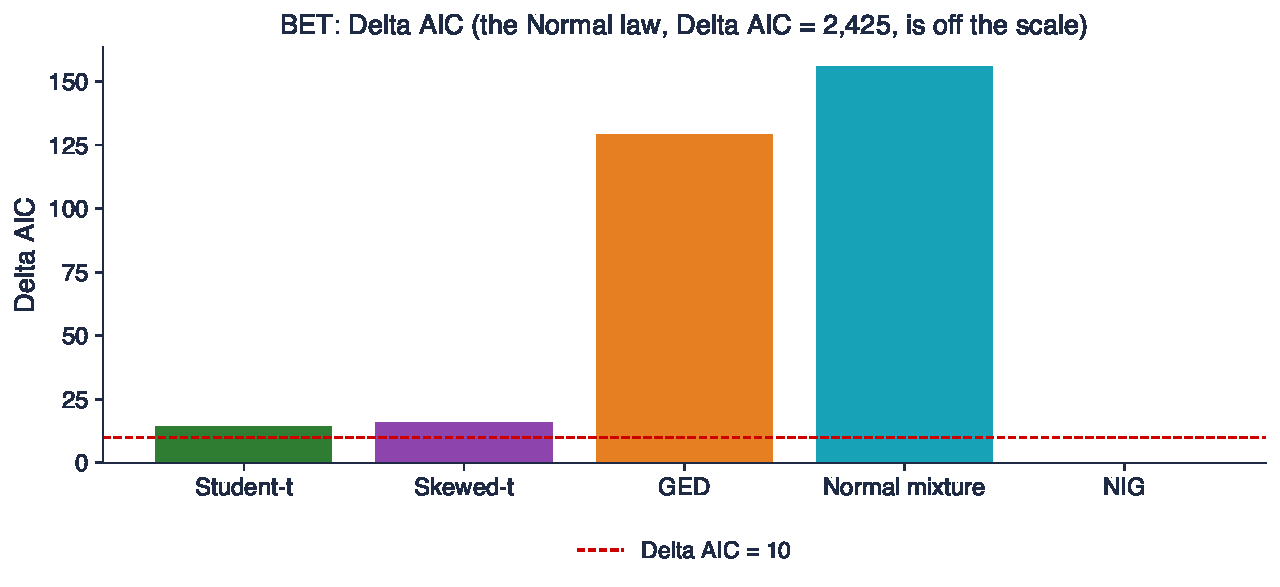
\includegraphics[width=0.96\textwidth,height=0.30\textheight,keepaspectratio]{ch6_sem_b1.pdf}
\end{center}
\vspace{-2mm}
\begin{center}
\tiny
\begin{tabular}{lrrrrrr}
\toprule
& $\ell(\hat\theta)$ & AIC & BIC & $\Delta$AIC & $\Delta$BIC & $w$ \\
\midrule
Normală & $-11\,702$ & $23\,407$ & $23\,421$ & $2425{,}2$ & $2411{,}6$ & $0{,}000$ \\
Student-t & $-10\,495$ & $20\,996$ & $21\,017$ & $14{,}4$ & $7{,}6$ & $0{,}001$ \\
skewed-t & $-10\,495$ & $20\,998$ & $21\,025$ & $16{,}0$ & $16{,}0$ & $0{,}000$ \\
GED & $-10\,553$ & $21\,111$ & $21\,132$ & $129{,}1$ & $122{,}3$ & $0{,}000$ \\
amestec Normal & $-10\,564$ & $21\,138$ & $21\,172$ & $155{,}8$ & $162{,}7$ & $0{,}000$ \\
NIG & $-10\,487$ & $20\,982$ & $21\,009$ & $0{,}0$ & $0{,}0$ & $0{,}999$ \\
\bottomrule
\end{tabular}
\end{center}
\begin{itemize}
    \item Cîștigător: NIG pe ambele criterii; Student-t $\hat\nu = 2{,}43$; skewed-t $\hat\lambda = -0{,}009$; $LR = 0{,}35$, $p = 0{,}555$: asimetria nu este necesară
    \item Interpretare: cozi foarte groase ($\nu$ aproape de 2) și nicio asimetrie semnificativă; legea Normală pierde la mii de puncte AIC
\end{itemize}\quantlet{SFM\_ch6\_seminar}{\qlurl{SFM_ch6_seminar}}
\end{frame}

\begin{frame}{B2: DAX și Bitcoin [Propus]}
\itemsize{\footnotesize}
\begin{itemize}
\item \textbf{Întrebarea}: aleg DAX și Bitcoin aceeași distribuție ca BET? Model: B1.
\item \textbf{Date}: DAX din 2000, Bitcoin din 2014 (7 zile pe săptămînă), randamente logaritmice zilnice în \%
\item \textbf{Cerințe}
\begin{enumerate}
    \item Repetați pașii 1--3 din B1 pentru fiecare serie.
    \item Spuneți dacă AIC și BIC sînt de acord pentru fiecare serie.
    \item Interpretare: de ce ar putea diferi cel mai bun model între un indice bursier și un activ cripto?
\end{enumerate}
\item \textbf{Raportați}: două tabele și trei fraze
\item Notebook: secțiunea B2
\end{itemize}
\end{frame}

\ifsolutions
\begin{frame}{B2: rezolvare [Propus]}
\itemsize{\footnotesize}
\begin{center}
\scriptsize
\begin{tabular}{lrrrrrr}
\toprule
& DAX $\Delta$AIC & DAX $\Delta$BIC & DAX $w$ & Bitcoin $\Delta$AIC & Bitcoin $\Delta$BIC & Bitcoin $w$ \\
\midrule
Normală & $1357{,}1$ & $1343{,}4$ & $0{,}000$ & $1429{,}5$ & $1423{,}1$ & $0{,}000$ \\
Student-t & $50{,}6$ & $43{,}8$ & $0{,}000$ & $94{,}6$ & $94{,}6$ & $0{,}000$ \\
skewed-t & $31{,}7$ & $31{,}7$ & $0{,}000$ & $96{,}1$ & $102{,}5$ & $0{,}000$ \\
GED & $44{,}8$ & $38{,}0$ & $0{,}000$ & $0{,}0$ & $0{,}0$ & $1{,}000$ \\
amestec Normal & $129{,}0$ & $135{,}8$ & $0{,}000$ & $158{,}6$ & $171{,}4$ & $0{,}000$ \\
NIG & $0{,}0$ & $0{,}0$ & $1{,}000$ & $28{,}5$ & $34{,}9$ & $0{,}000$ \\
\bottomrule
\end{tabular}
\end{center}
\begin{itemize}
    \item DAX: NIG (AIC și BIC); $LR$(Student-t vs skewed-t) $= 20{,}92$, $p <0{,}001$: asimetria este necesară, $\hat\lambda = -0{,}070$
    \item Bitcoin: GED (AIC și BIC), GED $\hat\beta = 0{,}80$; $LR = 0{,}42$, $p = 0{,}515$: fără asimetrie
    \item Interpretare: Bitcoin are un vîrf foarte ascuțit (multe zile liniștite) și altă formă a cozii; DAX are asimetria crahurilor, BET nu
\end{itemize}\quantlet{SFM\_ch6\_seminar}{\qlurl{SFM_ch6_seminar}}
\end{frame}
\fi

\begin{frame}{B3: trec cele mai bune modele? [Rezolvat]}
\itemsize{\footnotesize}
\begin{itemize}
\item \textbf{Întrebarea}: trec ajustările Normală și Student-t ale S\&P 500 testele KS, Cramér--von Mises și Anderson--Darling?
\item \textbf{Date}: randamentele logaritmice zilnice S\&P 500 din 2000 ($n = 6\,714$)
\item \textbf{Cerințe}
\begin{enumerate}
    \item Ajustați ambele modele și calculați cele trei statistici.
    \item Calculați valoarea $p$ KS naivă, care tratează parametrii ca fiind cunoscuți.
    \item Calculați valori $p$ prin bootstrap parametric cu $B = 99$ (simulare, reajustare, recalculare).
    \item Desenați graficul QQ al datelor față de ambele ajustări.
    \item Interpretare: dacă ambele modele sînt respinse, la ce mai folosește testul?
\end{enumerate}
\item \textbf{Raportați}: un tabel cu șase statistici și valorile $p$, graficul QQ și două fraze
\item Notebook: secțiunea B3
\end{itemize}
\end{frame}

\begin{frame}{B3: rezolvare [Rezolvat]}
\itemsize{\scriptsize}
\begin{center}
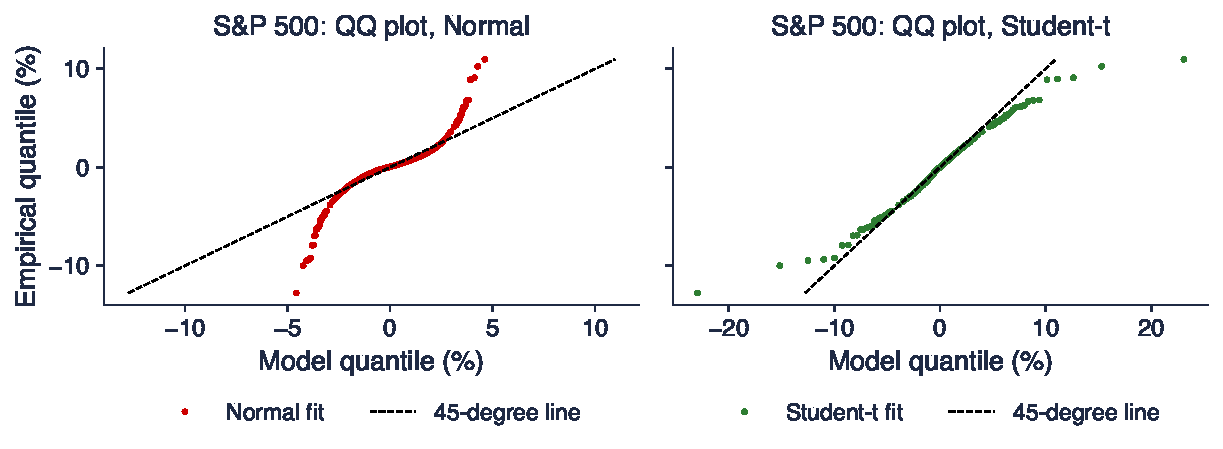
\includegraphics[width=0.96\textwidth,height=0.34\textheight,keepaspectratio]{ch6_sem_b3.pdf}
\end{center}
\vspace{-2mm}
\begin{center}
\tiny
\begin{tabular}{lrrrr}
\toprule
& KS & CvM & AD & $p$ KS naiv \\
\midrule
Normală & $0{,}093$ & $22{,}84$ & $127{,}35$ & $<0{,}001$ \\
valoare critică bootstrap 95\% & $0{,}011$ & $0{,}12$ & $0{,}75$ &  \\
Student-t & $0{,}018$ & $0{,}57$ & $4{,}69$ & $0{,}021$ \\
valoare critică bootstrap 95\% & $0{,}009$ & $0{,}08$ & $0{,}65$ &  \\
\bottomrule
\end{tabular}
\end{center}
\begin{itemize}
    \item $p$ bootstrap $= 0{,}01$ pentru fiecare statistică și ambele modele (cel mai mic posibil cu $B = 99$): ambele respinse; $p$ KS naiv al Student-t este mult prea mare
    \item Interpretare: cu $n = 6\,714$, orice model i.i.d.\ este respins; statisticile tot ordonează modelele (AD Student-t $4{,}69$ vs $127{,}35$), iar graficul QQ arată unde eșuează fiecare
\end{itemize}\quantlet{SFM\_ch6\_seminar}{\qlurl{SFM_ch6_seminar}}
\end{frame}

\begin{frame}{B4: crah sau eroare de date? Banca Transilvania [Propus]}
\itemsize{\scriptsize}
\begin{itemize}
\item \textbf{Întrebarea}: care dintre cele mai mari randamente TLV sînt reale și schimbă eliminarea celor greșite modelul ales? Model: B1.
\item \textbf{Date}: prețul ajustat TLV din 2010, randamente logaritmice zilnice în \%; prețul de închidere (neajustat) pentru comparație; BET în aceleași zile
\item \textbf{Cerințe}
\begin{enumerate}
    \item Listați cele mai mari trei randamente în valoare absolută, cu datele lor.
    \item Pentru fiecare, comparați prețul de închidere și prețul ajustat în jurul datei, precum și randamentul BET din aceeași zi.
    \item Decideți care zile sînt erori de date și eliminați doar acele zile.
    \item Reajustați cinci candidați; comparați aplatizarea, $\hat\nu$ Student-t, statistica AD și cîștigătorul AIC înainte și după.
    \item Interpretare: ce s-ar fi întîmplat dacă ați fi eliminat toate cele trei zile?
\end{enumerate}
\item \textbf{Raportați}: un tabel cu trei zile și verdictul vostru, un tabel înainte/după și două fraze
\item Notebook: secțiunea B4
\end{itemize}
\end{frame}

\ifsolutions
\begin{frame}{B4: rezolvare [Propus]}
\itemsize{\scriptsize}
\begin{itemize}
    \item Cele mai mari randamente absolute: 2016-05-30 ($-15{,}0\%$), 2016-05-31 ($20{,}5\%$), 2018-12-19 ($-22{,}2\%$)
    \begin{itemize}
        \item 30 mai 2016: prețul de închidere scade de la $2{,}83$ la $2{,}09$ (acțiuni gratuite), prețul ajustat doar de la $3{,}60$ la $3{,}10$, apoi sare la $3{,}81$: ajustarea are o zi întîrziere, \textbf{eroare de date}
        \item 19 decembrie 2018: prețul de închidere și cel ajustat scad amîndouă cu circa $20\%$, iar BET scade cu $-11{,}9\%$ în aceeași zi (taxa pe active bancare anunțată în decembrie 2018): un \textbf{crah real}, îl păstrăm
    \end{itemize}
    \item Înainte $\to$ după eliminarea celor două zile din mai 2016
    \begin{itemize}
        \item aplatizarea $20{,}5 \to 16{,}5$; abaterea standard $1{,}805 \to 1{,}758$; $\hat\nu$ Student-t $3{,}33 \to 3{,}44$; AD $1{,}29 \to 1{,}30$; cîștigătorul AIC Student-t $\to$ Student-t
    \end{itemize}
    \item Interpretare: eliminarea și a crahului real ar ascunde exact riscul pentru care este construit modelul; curățați doar erorile dovedite
\end{itemize}\quantlet{SFM\_ch6\_seminar}{\qlurl{SFM_ch6_seminar}}
\end{frame}
\fi

\begin{frame}{B5: VaR 1\% în afara eșantionului pentru DAX [Rezolvat]}
\itemsize{\scriptsize}
\begin{itemize}
\item \textbf{Întrebarea}: dă modelul ales de AIC pe 2000--2019 și cel mai bun VaR 1\% pe 2020--2026?
\item \textbf{Date}: randamentele logaritmice zilnice DAX: estimare 2000--2019 ($n = 5\,075$), test 2020--2026 ($n = 1\,710$)
\item \textbf{Cerințe}
\begin{enumerate}
    \item Ajustați cei șase candidați pe zilele de estimare și ordonați-i după AIC.
    \item Calculați scorul logaritmic mediu al fiecărui model pe zilele de test.
    \item Calculați VaR 1\% al fiecărui model, numărați depășirile pe zilele de test și aplicați testul Kupiec.
    \item Adăugați simularea istorică (cuantila de 1\% a zilelor de estimare) și VaR mediat cu ponderile Akaike.
    \item Interpretare: ce model ați alege pentru VaR 1\% și de ce?
\end{enumerate}
\item \textbf{Raportați}: un tabel, graficul și două fraze
\item Notebook: secțiunea B5
\end{itemize}
\end{frame}

\begin{frame}{B5: rezolvare [Rezolvat]}
\itemsize{\scriptsize}
\begin{center}
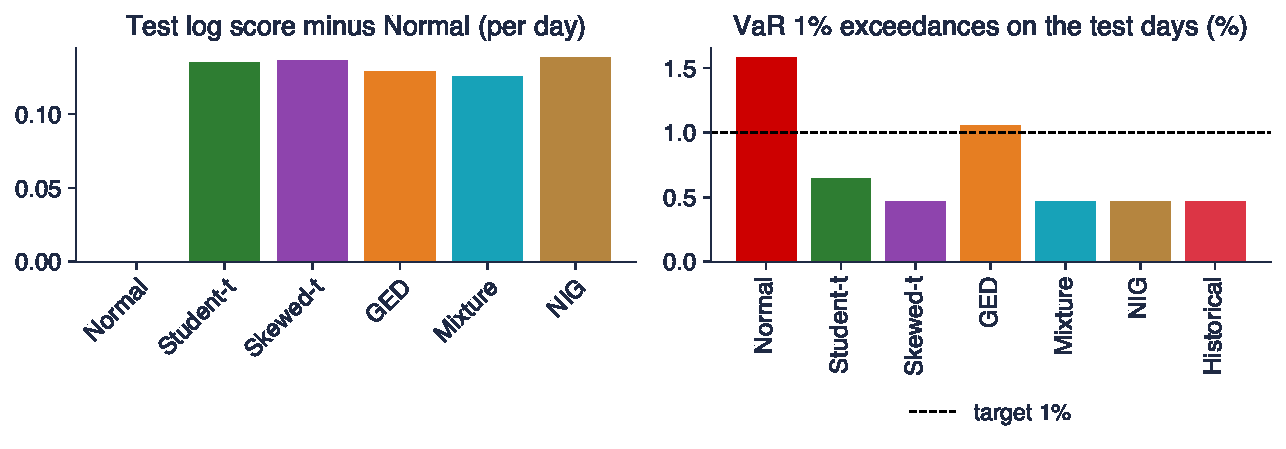
\includegraphics[width=0.96\textwidth,height=0.28\textheight,keepaspectratio]{ch6_sem_b5.pdf}
\end{center}
\vspace{-2mm}
\begin{center}
\tiny
\begin{tabular}{lrrrrr}
\toprule
& scor log. & VaR 1\% & depășiri & $p$ Kupiec & pinball $\times 100$ \\
\midrule
Normală & $-1{,}668$ & $3{,}37$ & 27 & $0{,}027$ & $5{,}37$ \\
Student-t & $-1{,}533$ & $4{,}09$ & 11 & $0{,}113$ & $5{,}23$ \\
skewed-t & $-1{,}532$ & $4{,}38$ & 8 & $0{,}014$ & $5{,}36$ \\
GED & $-1{,}539$ & $3{,}91$ & 18 & $0{,}828$ & $5{,}21$ \\
amestec Normal & $-1{,}542$ & $4{,}39$ & 8 & $0{,}014$ & $5{,}37$ \\
NIG & $-1{,}530$ & $4{,}38$ & 8 & $0{,}014$ & $5{,}36$ \\
istorică & -- & $4{,}33$ & 8 & $0{,}014$ & $5{,}33$ \\
mediată & -- & $4{,}37$ & 8 & $0{,}014$ & $5{,}36$ \\
\bottomrule
\end{tabular}
\end{center}
\begin{itemize}
    \item AIC pe 2000--2019: NIG; cel mai bun scor logaritmic de test: NIG; depășiri așteptate 17{,}1; cea mai mică pierdere pinball: GED
    \item Interpretare: cîștigătorul AIC dă cea mai bună densitate, dar prea puține depășiri (prea prudent); doar pentru VaR 1\%, GED și Student-t au fost mai aproape de 1\%
\end{itemize}\quantlet{SFM\_ch6\_seminar}{\qlurl{SFM_ch6_seminar}}
\end{frame}

\begin{frame}{B6: VaR 1\% în afara eșantionului pentru Bitcoin [Propus]}
\itemsize{\footnotesize}
\begin{itemize}
\item \textbf{Întrebarea}: se menține concluzia din B5 pentru Bitcoin? Model: B5.
\item \textbf{Date}: Bitcoin: estimare 2014--2019 ($n = 1\,931$), test 2020--2026 ($n = 2\,453$)
\item \textbf{Cerințe}
\begin{enumerate}
    \item Repetați pașii 1--4 din B5.
    \item Comparați VaR 1\% empiric al zilelor de test cu cel al zilelor de estimare.
    \item Interpretare: de ce eșuează aici toate modelele cu cozi groase testul Kupiec și în ce direcție?
\end{enumerate}
\item \textbf{Raportați}: un tabel și două fraze
\item Notebook: secțiunea B6
\end{itemize}
\end{frame}

\ifsolutions
\begin{frame}{B6: rezolvare [Propus]}
\itemsize{\footnotesize}
\begin{center}
\scriptsize
\begin{tabular}{lrrrrr}
\toprule
& scor log. & VaR 1\% & depășiri & $p$ Kupiec & pinball $\times 100$ \\
\midrule
Normală & $-2{,}605$ & $8{,}83$ & 23 & $0{,}754$ & $12{,}97$ \\
Student-t & $-2{,}443$ & $13{,}48$ & 7 & $<0{,}001$ & $15{,}36$ \\
skewed-t & $-2{,}443$ & $13{,}32$ & 7 & $<0{,}001$ & $15{,}24$ \\
GED & $-2{,}443$ & $11{,}33$ & 10 & $<0{,}001$ & $13{,}87$ \\
amestec Normal & $-2{,}462$ & $11{,}32$ & 10 & $<0{,}001$ & $13{,}87$ \\
NIG & $-2{,}438$ & $12{,}56$ & 7 & $<0{,}001$ & $14{,}70$ \\
istorică & -- & $11{,}39$ & 10 & $<0{,}001$ & $13{,}91$ \\
mediată & -- & $11{,}33$ & 10 & $<0{,}001$ & $13{,}87$ \\
\bottomrule
\end{tabular}
\end{center}
\begin{itemize}
    \item Depășiri așteptate 24{,}5; cel mai bun scor logaritmic de test: NIG; cea mai mică pierdere pinball: Normală
    \item VaR 1\% empiric al zilelor de test: $8{,}63\%$, față de $11{,}39\%$ pe zilele de estimare: Bitcoin a devenit mai calm
    \item Interpretare: toate modelele cu cozi groase sînt prea prudente (prea puține depășiri); modelul Normal trece din întîmplare: un model static ajustat pe un trecut agitat nu poate urmări un prezent mai calm
\end{itemize}\quantlet{SFM\_ch6\_seminar}{\qlurl{SFM_ch6_seminar}}
\end{frame}
\fi


%=============================================================================
\section{Partea C: întrebări deschise și critica unui răspuns AI}
%=============================================================================

\begin{frame}{C1: se schimbă în timp cel mai bun model? [Propus]}
\itemsize{\footnotesize}
\begin{itemize}
\item \textbf{Întrebarea}: este cîștigătorul AIC pentru S\&P 500 și BET același în fiecare fereastră de doi ani?
\item \textbf{Date}: randamente logaritmice zilnice din 2000, ferestre de doi ani care nu se suprapun (2000--2001, 2002--2003, ...); candidați: Normală, Student-t, skewed-t, GED, NIG; modele: B1, A1
\item \textbf{Cerințe}
\begin{enumerate}
    \item În fiecare fereastră, găsiți cîștigătorul AIC, ponderea lui Akaike și $\Delta$AIC al celui de-al doilea.
    \item Numărați de cîte ori cîștigă fiecare model, pentru fiecare indice.
    \item Propuneți o explicație a schimbărilor și o cale de a o testa.
    \item Interpretare: ar trebui un model de risc reselectat la fiecare doi ani?
\end{enumerate}
\item \textbf{Raportați}: un tabel, o numărătoare a cîștigătorilor și un plan de proiect
\item Notebook: secțiunea C1
\end{itemize}
\end{frame}

\ifsolutions
\begin{frame}{C1: analiză de referință [Propus]}
\itemsize{\scriptsize}
\begin{columns}[T]
\begin{column}{0.48\textwidth}
\centering S\&P 500\begin{center}
\tiny
\begin{tabular}{llrlr}
\toprule
fereastra & cîștigător & $w$ & al doilea & $\Delta$ \\
\midrule
2000--2001 & Student-t & $0{,}46$ & NIG & $1{,}7$ \\
2002--2003 & GED & $0{,}44$ & Student-t & $1{,}0$ \\
2004--2005 & Normală & $0{,}41$ & skewed-t & $1{,}5$ \\
2006--2007 & GED & $0{,}81$ & NIG & $3{,}0$ \\
2008--2009 & GED & $0{,}50$ & NIG & $0{,}3$ \\
2010--2011 & GED & $0{,}92$ & NIG & $5{,}1$ \\
2012--2013 & GED & $0{,}68$ & NIG & $3{,}0$ \\
2014--2015 & GED & $0{,}90$ & NIG & $5{,}1$ \\
2016--2017 & GED & $0{,}75$ & NIG & $2{,}3$ \\
2018--2019 & NIG & $0{,}83$ & GED & $4{,}1$ \\
2020--2021 & skewed-t & $0{,}48$ & Student-t & $0{,}2$ \\
2022--2023 & GED & $0{,}69$ & Student-t & $3{,}0$ \\
2024--2025 & skewed-t & $0{,}73$ & Student-t & $2{,}5$ \\
\bottomrule
\end{tabular}
\end{center}

\end{column}
\begin{column}{0.48\textwidth}
\centering BET\begin{center}
\tiny
\begin{tabular}{llrlr}
\toprule
fereastra & cîștigător & $w$ & al doilea & $\Delta$ \\
\midrule
2000--2001 & Student-t & $0{,}39$ & skewed-t & $0{,}3$ \\
2002--2003 & NIG & $0{,}83$ & GED & $3{,}9$ \\
2004--2005 & Student-t & $0{,}59$ & skewed-t & $1{,}6$ \\
2006--2007 & GED & $0{,}59$ & Student-t & $2{,}7$ \\
2008--2009 & NIG & $0{,}37$ & Student-t & $0{,}5$ \\
2010--2011 & Student-t & $0{,}71$ & skewed-t & $2{,}0$ \\
2012--2013 & Student-t & $0{,}66$ & skewed-t & $2{,}0$ \\
2014--2015 & Student-t & $0{,}68$ & skewed-t & $2{,}0$ \\
2016--2017 & Student-t & $0{,}65$ & skewed-t & $1{,}8$ \\
2018--2019 & Student-t & $0{,}67$ & skewed-t & $1{,}4$ \\
2020--2021 & Student-t & $0{,}53$ & skewed-t & $0{,}7$ \\
2022--2023 & skewed-t & $0{,}43$ & NIG & $0{,}4$ \\
2024--2025 & skewed-t & $0{,}52$ & NIG & $0{,}5$ \\
\bottomrule
\end{tabular}
\end{center}

\end{column}
\end{columns}\begin{itemize}
    \item S\&P 500: GED cîștigă 8 din 13 ferestre; BET: Student-t cîștigă 8 din 13; al doilea este adesea la $\Delta < 2$
    \item Cîștigătorul pe tot eșantionul (NIG) cîștigă rar în ferestre scurte: cu $n \approx 500$, candidații se separă greu, iar regimurile de volatilitate schimbă forma
    \item Direcții de proiect: standardizați întîi cu un model de volatilitate; ferestre mai lungi; mai multe piețe
\end{itemize}\quantlet{SFM\_ch6\_seminar}{\qlurl{SFM_ch6_seminar}}
\end{frame}
\fi

\begin{frame}{C2: verificați un răspuns AI [Propus]}
\itemsize{\scriptsize}
\begin{itemize}
    \item Un student a cerut unui asistent AI să aleagă o distribuție pentru randamentele logaritmice zilnice S\&P 500 (\%) din 2000 ($n = 6\,714$). Răspunsul:
    \item \aiprompt{(a) Skewed-t are cel mai mic AIC, deci este semnificativ mai bun decît Student-t (Delta AIC = 17{,}6).}
    \item \aiprompt{(b) Testul KS al ajustării Student-t dă p = 0{,}021 cu scipy.stats.kstest, deci Student-t se potrivește la nivelul de 1\%.}
    \item \aiprompt{(c) Testul LR Normală vs Student-t folosește valoarea critică chi2(1) 3,84.}
    \item \aiprompt{(d) BIC penalizează parametrii în plus mai puțin decît AIC, pentru că ln(n) este doar 8{,}81.}
    \item \aiprompt{(e) Testul Anderson-Darling este mai sensibil decît KS la potrivirea din cozi.}
    \item \aiprompt{(f) Pentru că skewed-t are cea mai bună potrivire, VaR 1\% al lui este cel mai precis.}
    \item Cerințe
    \begin{itemize}
        \item 1. Pentru fiecare afirmație spuneți dacă este corectă; dacă nu, dați afirmația corectă și, unde se poate, cifra corectă din notebook (secțiunea C2).
        \item 2. Raportați: o listă de șase verdicte, fiecare cu un rînd de justificare.
    \end{itemize}
\end{itemize}
\end{frame}

\ifsolutions
\begin{frame}{C2: rezolvare [Propus]}
\itemsize{\footnotesize}
\begin{itemize}
    \item (a) Formulare greșită: AIC nu este un test și nu are „semnificație”; un $\Delta$AIC de $17{,}6$ este o dovadă puternică după regulile practice (testul LR pentru $\lambda = 0$ este de acord)
    \item (b) Greșit: parametrii au fost estimați pe aceleași date, deci $p$ KS naiv este prea mare; un bootstrap parametric dă $p \le 0{,}01$, iar $p = 0{,}021 < 0{,}05$ oricum
    \item (c) Greșit: $1/\nu = 0$ este la frontieră; valoarea critică corectă la 5\% este $2{,}71$ (decizia nu se schimbă: $LR = 1\,949$)
    \item (d) Greșit: $\ln n = 8{,}81 > 2$, deci BIC penalizează fiecare parametru de peste patru ori mai mult decît AIC
    \item (e) Corect: AD ponderează pătratul distanței cu $1/[F(1 - F)]$, mare în cozi
    \item (f) Logică greșită: cea mai bună potrivire globală nu implică cea mai bună cuantilă; în eșantion, VaR 1\% skewed-t este $3{,}71\%$, Student-t $3{,}46\%$, datele $3{,}45\%$; judecați VaR după depășirile din afara eșantionului
\end{itemize}\quantlet{SFM\_ch6\_seminar}{\qlurl{SFM_ch6_seminar}}
\end{frame}
\fi


%=============================================================================
\section{Încheiere}
%=============================================================================

\begin{frame}{Idei de reținut}
\itemsize{\small}
\begin{itemize}
    \item AIC și BIC ordonează modelele; $\Delta \le 2$ înseamnă egalitate; ponderile Akaike transformă $\Delta$ în dovezi
    \item Testele LR cer modele imbricate și un parametru în interiorul spațiului; la frontieră folosiți amestecul 50:50
    \item KS cu parametri estimați cere Lilliefors sau bootstrap; AD vede cozile, KS nu
    \item Verificați cele mai mari randamente înainte de modelare: eliminați erorile, păstrați crahurile
    \item Cea mai bună densitate nu dă întotdeauna cel mai bun VaR: validați în afara eșantionului
\end{itemize}
\end{frame}

\begin{frame}{După seminar}
\itemsize{\small}
\begin{itemize}
    \item Cursul 6 dezvoltă fiecare temă de azi: verosimilitatea, testele LR și Vuong, AIC și BIC, testele EDF, graficele QQ, VaR în afara eșantionului, incertitudinea de model
    \item Încercați cerințele [Propus] în notebook; rezolvările se discută la seminar
    \item C1 poate deveni un proiect de echipă: randamente standardizate, mai multe piețe, ferestre mobile
    \item Lectură: \refBA; \refStephens; \refKupiec
\end{itemize}
\end{frame}


%=============================================================================
\section{Bibliografie}
%=============================================================================

\begin{frame}{Bibliografie}
\itemsize{\tiny}
\begin{itemize}
    \item Akaike, H. (1974). \href{https://doi.org/10.1109/TAC.1974.1100705}{A new look at the statistical model identification}. \textit{IEEE Transactions on Automatic Control}, 19(6), 716--723.
    \item Burnham, K.P., Anderson, D.R. (2004). \href{https://doi.org/10.1177/0049124104268644}{Multimodel inference: understanding AIC and BIC in model selection}. \textit{Sociological Methods \& Research}, 33(2), 261--304.
    \item Franke, J., Härdle, W.K., Hafner, C.M. (2019). \href{https://doi.org/10.1007/978-3-030-13751-9}{\textit{Statistics of Financial Markets: An Introduction}}, 5th ed. Springer.
    \item Hansen, B.E. (1994). \href{https://doi.org/10.2307/2527081}{Autoregressive conditional density estimation}. \textit{International Economic Review}, 35(3), 705--730.
    \item Kupiec, P.H. (1995). \href{https://doi.org/10.3905/jod.1995.407942}{Techniques for verifying the accuracy of risk measurement models}. \textit{Journal of Derivatives}, 3(2), 73--84.
    \item Lilliefors, H.W. (1967). \href{https://doi.org/10.1080/01621459.1967.10482916}{On the Kolmogorov--Smirnov test for normality with mean and variance unknown}. \textit{Journal of the American Statistical Association}, 62(318), 399--402.
    \item Schwarz, G. (1978). \href{https://doi.org/10.1214/aos/1176344136}{Estimating the dimension of a model}. \textit{Annals of Statistics}, 6(2), 461--464.
    \item Self, S.G., Liang, K.-Y. (1987). \href{https://doi.org/10.1080/01621459.1987.10478472}{Asymptotic properties of maximum likelihood estimators and likelihood ratio tests under nonstandard conditions}. \textit{Journal of the American Statistical Association}, 82(398), 605--610.
    \item Stephens, M.A. (1974). \href{https://doi.org/10.1080/01621459.1974.10480196}{EDF statistics for goodness of fit and some comparisons}. \textit{Journal of the American Statistical Association}, 69(347), 730--737.
    \item Wilks, S.S. (1938). \href{https://doi.org/10.1214/aoms/1177732360}{The large-sample distribution of the likelihood ratio for testing composite hypotheses}. \textit{Annals of Mathematical Statistics}, 9(1), 60--62.
\end{itemize}
\end{frame}

\end{document}
